%%%%%%%%%%%%%%%%%%%%%%%%%%%%%%%%%%%%%%%%%%%%%%%%%%%%%%%%%%%%%%%%%%%%%%%%%%%%%%%%%%%%%%%%%%%%%%%%%%%%%%%%%%%%%%%%%%%%%%%%%%%%%%%%%%%%%%%%%%%%%%%%%%%%%%%%%%%
% This is just an example/guide for you to refer to when submitting manuscripts to Frontiers, it is not mandatory to use Frontiers .cls files nor frontiers.tex  %
% This will only generate the Manuscript, the final article will be typeset by Frontiers after acceptance.   
%                                              %
%                                                                                                                                                         %
% When submitting your files, remember to upload this *tex file, the pdf generated with it, the *bib file (if bibliography is not within the *tex) and all the figures.
%%%%%%%%%%%%%%%%%%%%%%%%%%%%%%%%%%%%%%%%%%%%%%%%%%%%%%%%%%%%%%%%%%%%%%%%%%%%%%%%%%%%%%%%%%%%%%%%%%%%%%%%%%%%%%%%%%%%%%%%%%%%%%%%%%%%%%%%%%%%%%%%%%%%%%%%%%%

%%% Version 3.4 Generated 2018/06/15 %%%
%%% You will need to have the following packages installed: datetime, fmtcount, etoolbox, fcprefix, which are normally inlcuded in WinEdt. %%%
%%% In http://www.ctan.org/ you can find the packages and how to install them, if necessary. %%%
%%%  NB logo1.jpg is required in the path in order to correctly compile front page header %%%

\documentclass[utf8]{frontiersSCNS} % for Science, Engineering and Humanities and Social Sciences articles
%\documentclass[utf8]{frontiersHLTH} % for Health articles
%\documentclass[utf8]{frontiersFPHY} % for Physics and Applied Mathematics and Statistics articles

%\setcitestyle{square} % for Physics and Applied Mathematics and Statistics articles
\usepackage{url,hyperref,lineno,microtype,subcaption}
\usepackage[onehalfspacing]{setspace}
\usepackage[utf8]{vietnam}
\usepackage{hyperref}
\usepackage{placeins}
%\linenumbers


% Leave a blank line between paragraphs instead of using \\


\def\keyFont{\fontsize{8}{11}\helveticabold }
\def\firstAuthorLast{22-03-2023} %use et al only if is more than 1 author
\def\Authors{Lê Thanh Nam\,$^{1,*, 2, 3, 4}$}
%\def\Authors{Lê Thanh Nam\,$^{1,*}$, Co-Author\,$^{2}$ and Co-Author\,$^{1,2}$}
% Affiliations should be keyed to the author's name with superscript numbers and be listed as follows: Laboratory, Institute, Department, Organization, City, State abbreviation (USA, Canada, Australia), and Country (without detailed address information such as city zip codes or street names).
% If one of the authors has a change of address, list the new address below the correspondence details using a superscript symbol and use the same symbol to indicate the author in the author list.
\def\Address{$^{1}$Tiến Sĩ, Kĩ Sư Xây Dựng: Viện Đô Thị Thông Minh và Quản Lý (ISCM), Trường Công Nghệ và Thiết Kế, Đại Học UEH, tp. Hồ Chí Minh -  \href{https://www.iscm.ueh.edu.vn/}{www.iscm.ueh.edu.vn} \\
$^{2}$Giám Đốc Kĩ Thuật, Chuyên Gia Soạn Hợp Đồng (FIDIC): Công Ty Tư Vấn ARCADIS, phụ trách thị trường Đông Nam Á và Ấn Độ -  \href{www.arcadis.com}{www.arcadis.com}\\
$^{3}$Giám Đốc: Công ty TNHH ASQ Việt Nam - \href{https://www.asq.vn}{www.asq.vn}\\
$^{4}$Cố Vấn Kĩ Thuật: Công ty EMAPTA - \href{www.emapta.com}{www.emapta.com}}
% The Corresponding Author should be marked with an asterisk
% Provide the exact contact address (this time including street name and city zip code) and email of the corresponding author
\def\corrAuthor{Di Động: +84-9-8378-0100 (Việt Nam) / +91-98-1044-4723 (Ấn Độ) Email: namlt@ueh.edu.vn}

%\def\corrEmail{Email: namlt@ueh.edu.vn}




\begin{document}
\onecolumn
\firstpage{1}

\title[Ứng Dụng Dữ Liệu Lớn/Quản Lý Hạ Tầng - Điện Lực]{Ứng Dụng Dữ Liệu Lớn và Quản Lý Tài Sản Hạ Tầng Trong Ngành Điện Lực} 

\author[\firstAuthorLast ]{\Authors} %This field will be automatically populated
\address{} %This field will be automatically populated
\correspondance{} %This field will be automatically populated

\extraAuth{}% If there are more than 1 corresponding author, comment this line and uncomment the next one.
%\extraAuth{corresponding Author2 \\ Laboratory X2, Institute X2, Department X2, Organization X2, Street X2, City X2 , State XX2 (only USA, Canada and Australia), Zip Code2, X2 Country X2, email2@uni2.edu}


\maketitle


\begin{abstract}
%Bài viết này tổng hợp 
Ngành điện lực là một trong những ngành xương sống cho sự phát triển kinh tế của quốc gia. Trong những năm gần đây, các công ty điện lực đã chứng kiến và trải nghiệm nhiều thử thách và sự đổi mới trong cả kĩ thuật và quản lý, và phần nào đã có những bước tiến đáng kể trong công tác chuyển đổi số (digitization) cùng với khái niệm về hệ thống truyền tải điện thông minh(Smart Grids). Các hệ thống điện thường luôn hoạt động trong tình trạng áp lực, chủ yếu là do sự gia tăng hàng năm trong nhu cầu sử dụng điện, sự thiếu hụt về nguồn cung về nhiên liệu/năng lượng để sản xuất ra điện, và các ràng buộc về môi trường áp đặt lên hệ thống sản xuất điện và sự mở rộng các đường dây tải điện. 

Ở Việt Nam, Tập Đoàn Điện Lực Việt Nam (EVN) cùng các bộ ngành liên quan đã soạn thảo và đề xuất "Qui Hoạch Điện 8 - PDP8" hướng tới sự phát triển ổn định và bền vững chiến lược đến năm 2050. Một trong những nội dung quan trọng của PDP8 có chú trọng đến việc phát triển và nâng cao khả năng ứng dụng các công nghệ tiên tiến và áp dụng dữ liệu lớn cũng như trí thông minh nhân tạo vào công tác xây dựng, điều hành và quản lý các hệ thống điện.

Bài viết này cung cấp cho người đọc một cái nhìn tổng quan về các ứng dụng phân tích dữ liệu lớn, công tác quản lý cơ sở hạ tầng trong ngành điện lực, và các vấn đề liên quan đến việc triển khai. Chú trọng của bài viết sẽ là các ứng dụng mới đã mang lại giá trị tích cực trong ngành, một số bài học rút ra từ việc triển khai ứng dụng tại một số tổ chức, và một số ý tưởng và chủ đề cần khám phá. Tổng quan các nghiên cứu khoa học trong ngành khoa học dữ liệu trong ngành điện sẽ được đề cập nhằm tạo ra được cái nhìn tổng quát cho việc ứng dụng và tiếp tục phát triển của ngành trong tương lai. Cuối cùng, bài viết nêu ra các cơ hội và thách thức cũng như các mục tiêu và chiến lược để đạt được các kết quả có ý nghĩa.


%Bài viết này chú trọng đến vài trò của công tác phân tích dữ liệu lớn và vai trò của công tác quản lý cơ sở hạ tầng trong các lĩnh vực quan trọng của nền kinh tế, đặc biệt chú trọng tới ngành điện. Nội dung bài viết đề cập đến việc sử dụng các nguồn cung cấp dữ liệu lớn mà rất khó có thể truy cập vào các hệ thống cơ sở dữ liệu tiêu chuẩn, việc quản lý và quan trắc trong ngành điện. Đảm bảo sự ổn định của hệ thống thông qua việc sử dụng hiệu quả các nguồn dữ liệu lớn là một trong những mục tiêu quan trọng của các công ty điện lực.


\tiny
 \keyFont{ \section{Từ Khóa:} Dữ Liệu Lớn, Quản Lý Tài Sản, Cơ Sở Hạ Tầng, Độ Tin Cậy, Trí Thông Minh Nhân Tạo, Rủi Do, Tổn Thương, Nguy Cơ} %All article types: you may provide up to 8 keywords; at least 5 are mandatory.
\end{abstract}

\section{Giới Thiệu}
%For Original Research Articles \citep{conference}, Clinical Trial Articles \citep{article}, and Technology Reports \citep{patent}, the introduction should be succinct, with no subheadings \citep{book}. For Case Reports the Introduction should include symptoms at presentation \citep{chapter}, physical exams and lab results \citep{dataset}.

Có rất nhiều định nghĩa và cách hiểu khác nhau về phân tích dữ liệu lớn trong các ứng dụng ngành điện, đặc biệt là công tác sản xuất, truyền tải, và phân phối. Điều này chủ yếu là vì lý do có khá nhiều cách tiếp cận trong ngành khoa học dữ liệu và mục đích rộng liên quan (ví dụ như việc sử dụng các công cụ toán xác xác thống kê, trí thông minh nhân tạo (AI), học máy). Tính phức tạp và đa dạng của phân tích dữ liệu lớn trong ngành còn đến từ nhiều cách thức ứng dụng trong các lĩnh vực như quản lý tài sản (Asset Management), điều hành, điều khiển hệ thống, an toàn và an ninh, các quyết định lập kế hoạch và thị trường. Trong đó, có một vấn đề nền tảng làm cho công tác phân tích dữ liệu lớn trong ngành điện lực đặc biệt khó khăn là liên quan đến dung lượng của dữ liệu. Dung lượng của dữ liệu trong ngành thường ở cấp độ Terabyte, lớn hơn rất nhiều cấp độ Petabyte là cấp độ đã được coi là lớn trong các lĩnh vực khác. Cuối cùng, khái niệm "phân tích dữ liệu" còn là khá mơ hồ và đôi khi bị hiểu sai bởi vì hầu hết các ứng dựng cơ bản hay ứng dụng truyền thống trong ngành điện là dựa trên việc xử lý các dữ liệu được đo đạc (measurement data). Công việc xử lý truyền thống này đôi khi không được coi là phân tích dữ liệu lớn trong ngành khoa học dữ liệu. Ví dụ như, các phương pháp truyền thống liên quan đến tính toán ước lượng trạng thái (state estimation) hay vị trí sự cố (outage location) thường không được coi là phân tích dữ liệu lớn nếu công tác phân tích này chỉ đơn thuần dựa vào các phương trình/công thức toán được phát triển trên nền tảng vật lý. Trong khi đó, ở một khía cạnh khác, việc phán đoán sự cố dựa trên các mô hình nền tảng dữ liệu sử dụng các dữ liệu về thời tiết và mất điện có độ phân giải cao thì được coi là phân tích dữ liệu lớn.

Bài viết này không chú trọng đến việc đưa ra một định nghĩa rành mạch về phân tích dữ liệu lớn trong ngành điện mà chỉ chú trọng đến việc tổng quan hóa và nêu ra một số nghiên cứu và ứng dụng gần nhất sử dụng các phương pháp tiên tiến trong ngành khoa học dữ liệu trong ngành điện, đặc biệt chú trọng đến công tác quản lý tài sản cơ sở hạ tầng ngành điện, quản lý sự cố, và tính tích hợp với năng lượng tái tạo.

Có thể nói, một trong những bài báo nghiên cứu đầu tiên liên quan đến việc ứng dụng dữ liệu lớn trong ngành điện là bài báo của tác giả \cite{Kezunovic2013}. Tuy nhiên, nghiên cứu này chỉ dừng lại ở dạng mô hình và lý thuyết mà chưa đưa ra ứng dụng cụ thể vào thực tế. Việc ứng dụng vào thực tế mới chỉ được tiến hành trong vài năm gần đây.

Với mục đích hướng tới việc truyền tải kiến thức và đào tạo, ở bài viết này, một số khái niệm cơ bản cấu thành nên công tác phân tích dữ liệu lớn trong ngành điện và các khía cạnh đặc thù của ngành điện sẽ được đề cập. 

\section{Tầm Quan Trọng và Tính Khả Thi của Phân Tích Dữ Liệu Lớn trong Ngành Điện}
\subsection{Sự Tác Động của Phân Tích Dữ Liệu Lớn}

Sự thay đổi mạnh mẽ trong ngành điện dường như là chưa có tiền lệ, bao gồm sự chuyển dịch trong phân bổ tỷ lệ các dạng năng lượng (Energy Mix), yêu cầu và nhu cầu ngành càng cao của khách hàng, sự xuất hiện các kĩ thuật tiên tiến và thiết bị mới, và các mô hình kinh doanh mới. Chính những thay đổi này dẫn đến tính phức tạp (Complexity) và tính không chắc chắn (Uncertainty), cũng như mang tới các thách thức và cơ hội mới. Ở trung tâm của việc giải quyết các thách thức chính là việc đưa ra các quyết định tốt hơn và tối ưu hơn trong giai đoạn vận hành và lập kế hoạch, bao gồm cả công tác đầu tư dài hạn và phát triển chính sách.

Như chúng ta đã biết, lưới điện thông minh ngày nay đã và đang tiếp tục được trang bị các thiết bị tiên tiến có khả năng cảm biến (sensing) và thu thập dữ liệu với độ phân giải cao hơn nhiều so với trước đây. Dữ liệu mới kèm theo các phương pháp phân tích mới có thể hỗ trợ các mục tiêu trong quản lý hệ thống điện như việc đạt được độ bền thiết bị cao hơn, hiệu quả kinh tế tốt hơn và giảm khí thải. 

Phân tích dữ liệu vì thế trở thành một phần quan trọng giúp doanh nghiệp nâng cao khả năng ứng dụng các công nghệ hiện có nhằm đưa ra các quyết định tối ưu hơn. Các ứng dụng của phân tích dữ liệu cho ngành điện là rất nhiều và có thể được xác định trong nhiều hoạt động của ngành. Do đó, phân tích dữ liệu lớn đã, đang và sẽ là một bước đổi mới quan trọng trong đối trong các tổ chức cơ quan ngành điện lực.

\subsection{Nguồn Dữ Liệu}
Việc áp dụng các giải pháp phân tích dữ liệu lớn trong các hệ thống phân phối và truyền tải điện khác nhau thường được tập trung vào việc khai thác các nguồn dữ liệu không có tính đồng nhất (heterogeneous), là các khối dữ liệu có chất lượng riêng biệt, độ phân giải không gian/và thời gian khách nhau, và có cách trình bày thông tin khác nhau. Sẽ là khả thi để nâng cao ứng dụng nguồn dữ liệu này thông qua các phương pháp như: (a) kết hợp các nguồn dữ liệu mới và nguồn dữ liệu truyền thống, ví dụ thông qua việc sử dụng lý thuyết hợp nhất dữ liệu (data fusion) \citep{SimoesCosta2013}; (b) trích xuất và kết hợp thông tin từ các dữ liệu có định dạng khác nhau (ví dụ như dữ liệu ở hạng ảnh và ở dạng văn bản) thông qua các mô hình đa chiều (multimodal learning) \citep{Srivastava2012} hoặc qua một mạng lưới thông tin có tính không đồng nhất (heterogeneous) \citep{Sun2016}; và (c) kết hợp dữ liệu từ các nguồn dữ liệu phân tán về mặt địa lý, ví dụ như việc sử dụng các phương pháp Vector Autoregressive (VAR) truyền thống \citep{Cavalcante2017} hay phương pháp học sâu (Deep Learning) \citep{Zhu2020}.

Nguồn dữ liệu đến từ các lĩnh vực khác nhau:

\begin{itemize}
	\item \textbf{Hạ tầng mạng lưới điện}: Các doanh nghiệp quản lý và điều hành hệ thống đang cải thiện và nâng cao khả năng quan sát của hệ thống mạng bằng cách lắp đặt các đơn vị đo pha (PMU) có thể cung cấp dữ liệu với tốc độ báo cáo cao (ví dụ, 30 đơn vị đo lường trên mỗi giây của độ lớn điện áp/dòng điện, pha và tần số) và các thiết bị đầu cuối điểm từ xa (Remote Terminal Units - RTU) tại các trạm biến áp và các công tơ điện thông minh lắp đặt cho khách hàng. Các cảm biến được dùng cho việc giám sát từ xa các trạm biến áp cũng đang được thử nghiệm để theo dõi tình trạng làm việc của thiết bị và cải thiện chất lượng dịch vụ \citep{Leitao2015}.
	
	\item \textbf{Nhà máy điện tái tạo}: Các nhà máy sản xuất điện năng lượng tái tạo đang tiến hành lắp đặt và vận hành các cảm biến giám sát trong turbin và trong các cánh quạt (có những trường hợp lên đến hàng trăm cảm biến), các cảm biến này thu nhập hơn 10.000 điểm dữ liệu mỗi giây). Các dữ liệu này có thể được dùng cho công tác dự đoán sự cố và bảo trì thiết bị (giảm chi phí vận hành và bảo trì; dữ liệu từ mạng lưới dự báo thời tiết số, các cảm biến phân tán địa lý (ví dụ, cánh quạt điện gió, các cảm biến đo độ chiếu sáng), máy ảnh ghi lại bầu trời và hình ảnh vệ tinh có thể được kết hợp để cải thiện khả năng dự báo công suất (và thời tiết) trong nhiều khung thời gian khác nhau \citep{Sweeney2020}. Trong việc dự báo điện năng tái tạo, quy mô kết nối và sử dụng dữ liệu cũng đã tăng từ một địa điểm đến hàng trăm địa điểm \citep{Messner2019}.
	
	\item \textbf{Người tiêu dùng và mạng xã hội}: trong khi đang ở giai đoạn đầu của triển khai, sự lan rộng của các thiết bị liên kết Internet trong các căn hộ và tòa nhà thông minh đang tạo điều kiện cho các dịch vụ về năng lượng và phi năng lượng dựa trên dữ liệu \citep{Ahmed2016}, ảnh hưởng của chúng phụ thuộc vào việc giải quyết các thách thức như bảo vệ/quyền riêng tư dữ liệu và tương tác với người tiêu dùng. Hơn nữa, sự gia tăng của mạng xã hội đã cho phép các công ty điện lực hiểu và tương tác với khách hàng tốt hơn trước rất nhiều\citep{MorenoMunoz2016}. Các nhà nghiên cứu cũng đã thử kết hợp dữ liệu Twitter vào việc phát hiện cục bộ mất điện \citep{Sun2016}.
	
	\item \textbf{Thị trường điện}: Trong vài năm qua, đặc biệt tại châu Âu, tính minh bạch của thị trường điện đã được cải thiện đáng kể, và sau khi xuất bản Quy định (EU) số 543/2013 \citep{EU2013}, lượng dữ liệu công khai có sẵn đang tăng lên \citep{Hirth2018}, bao gồm cả truy cập vào các đề xuất riêng lẻ từ các công ty cung cấp điện trên thị trường (thông thường có sẵn với độ trễ vài tháng). Cùng xu hướng đó đang diễn ra ở Mỹ, với các nền tảng như bộ sưu tập dữ liệu Form EIA-930 cung cấp nguồn dữ liệu toàn diện và tập trung cho các dữ liệu hoạt động hàng giờ của lưới điện cao áp tại 48 tiểu bang. Dữ liệu mở này có thể được sử dụng cho các mục đích khác nhau: cải thiện kỹ năng dự báo giá điện bằng cách kết hợp phân tích giá điện từ các khu vực khác nhau \citep{Ziel2018} hoặc đánh giá ảnh hưởng quy mô lớn của việc phát điện từ nguồn năng lượng tái tạo được cấp bởi lưới điện liên kết với các quốc gia láng giềng \citep{Zugno2013}.
	
	\item \textbf{Môi trường và thời tiết}: Dữ liệu thời tiết đóng vai trò quan trọng trong việc dự đoán điều kiện hoạt động, bao gồm cả lỗi hỏng hóc thiết bị và đường dây. Dữ liệu từ các trạm thời tiết trên mặt đất, vệ tinh và tài nguyên radar có sẵn từ cơ sở dữ liệu của chính phủ. Mạng lưới cảm biến chuyên dụng, chẳng hạn như mạng lưới phát hiện sét quốc gia ở Mỹ, cũng là nguồn cung cấp dữ liệu thời tiết khá hữu ích. Nhiều dịch vụ dự báo thời tiết cũng có sẵn để cung cấp các tính năng được tính trước của các tập dữ liệu thời tiết. Ngoài ra, dữ liệu về rừng và nông nghiệp, đất đai, di cư động vật và các điều kiện xung quanh khác cũng có thể có sẵn từ nhiều nguồn khác nhau. Cách sử dụng dữ liệu chính xác cao bằng cách sử dụng các cơ sở dữ liệu chuyên dụng như hệ thống (LIDAR - Light Detection and Ranging) hoặc khảo sát bằng thiết bị bay drone cũng được nghiên cứu và đưa vào thực tiễn. Những dữ liệu này thường không được thu thập trong phạm vi chức năng của ngành điện nhưng chúng lại là một nguồn dữ liệu quan trọng cho ngành này. Chẳng hạn, trong dự báo tải, các nghiên cứu đã chuyển từ việc sử dụng nhiệt độ được thu thập tại một trạm đến nhiều biến thời tiết và nhiều trạm thời tiết \citep{Hong2015}. Trong dự báo điện mặt trời, dữ liệu hình ảnh bầu trời được sử dụng nhiều để phát hiện đám mây \citep{Kleissl2013}.
\end{itemize}
Các nhà nghiên cứu và chuyên gia hiện nay tập trung vào việc khai thác dữ liệu hiện có và khám phá các nguồn dữ liệu mới và dữ liệu với quy mô lớn để theo đuổi các cải tiến trong lập kế hoạch và vận hành lưới điện. Có nhiều khía cạnh quan trọng khác của phân tích dữ liệu lớn, chẳng hạn như xây dựng thuật toán có thể tận dụng môi trường tính toán hiệu suất cao và mở rộng kích thước mô hình để nắm bắt các đặc trưng chi tiết trong dữ liệu \citep{Wang2016}. Một ví dụ khác là sử dụng dữ liệu tải và thời tiết hàng giờ để dự báo tải dài hạn, thông thường dựa trên dữ liệu hàng tháng \citep{Hyndman2009,Hong2014}. Một bài đánh giá gần đây về phân tích dữ liệu lấy từ các công tơ thông minh liệt kê 10 bộ dữ liệu công khai về nhu cầu điện \citep{Wang2018}. Hình \ref{fig:1} là một ví dụ mô tả các thuộc tính cơ bản của dữ liệu lớn trong ngành điện.

\FloatBarrier
\begin{figure}[h]
\centering
	\begin{center}
		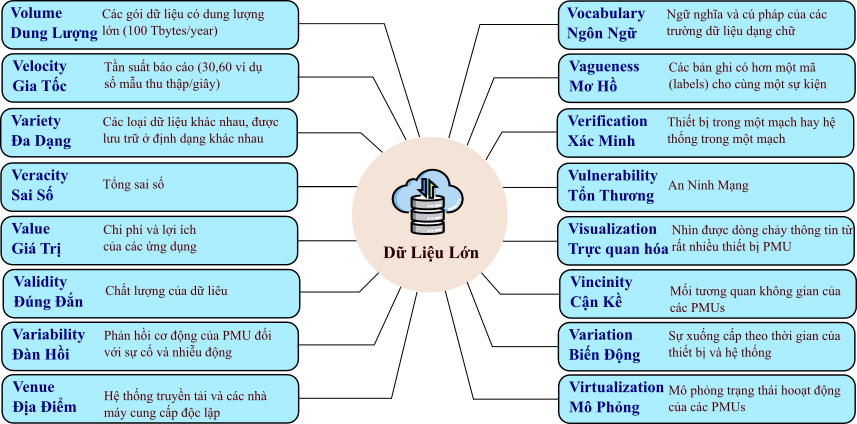
\includegraphics[width=\textwidth]{big-data-properties-VN}% This is a *.eps file
	\end{center}
	\caption{Các thuộc tính cơ bản của dữ liệu lớn trong ngành điện}\label{fig:1}
\end{figure}
\FloatBarrier


\subsection{Một Số Lưu Ý Quan Trọng Khi Tạo Ra Các Tập Dữ Liệu}

Cách tạo các tập dữ liệu như thế nào là khá quan trọng để sử dụng và ứng dụng các công cụ phân tích dữ liệu lớn. Một số cân nhắc sau cần được quan tâm khi thiết lập, tạo lập, và thu thập các gói dữ liệu: 

\begin{itemize}
\item Tính đồng bộ và mối tương quan theo không gian và thời gian
\item Tính mở rộng
\item Dữ liệu trống
\item Sự đa dạng của dữ liệu xấu
\item Các loại dữ liệu có độ tin cậy thấp/có tính biến thiên cao
\end{itemize}

Cách mà mỗi yếu tố này phản ánh lên các ứng dụng dữ liệu lớn trong lưới điện nằm ngoài phạm vi của bài viết này, nhưng chắc chắn đáng khám phá khi các tập dữ liệu mới được thêm vào và kết hợp với nhau trong quá trình xử lý và phân tích.

\section{Thách Thức của Công Việc Phân Tích Dữ Liệu Lớn}
\subsection{Nền Tảng của Khoa Học Dữ Liệu}
Mục tiêu của khoa học dữ liệu là trích xuất giá trị từ dữ liệu. Các bước của vòng đời quản lý dữ liệu bao gồm thu thập dữ liệu; tiền xử lý (khám phá, lấy mẫu, giảm chiều/thu gọn các đặc trưng và thuộc tính, tạo đặc trưng và thuộc tính, biến đổi, làm sạch và tích hợp); xử lý phân tích (mô hình hóa, thường bao gồm nhiều khối mô hình xây dựng liên kết với nhau); giải thích và báo cáo kết quả \citep{Aggarwal2015}. Những kỹ năng chính cần thiết trong lĩnh vực này thường được xem là đa ngành ở giao điểm của khoa học máy tính, toán học, thống kê và các lãnh vực khoa học kĩ thuật và xã hội khác (Hình \ref{fig:khoahocdulieu01}). Trên mặt kỹ thuật, các thách thức chính thường liên quan đến dữ liệu lớn, trí thông minh nhân tạo và các phương pháp học máy, trong khi quá trình khoa học dữ liệu áp dụng cũng có thể yêu cầu các kỹ năng khoa học xã hội, giao tiếp và kinh doanh (Hình \ref{fig:khoahocdulieu02}).

\FloatBarrier
\begin{figure}[h]
	\centering
	\begin{center}
		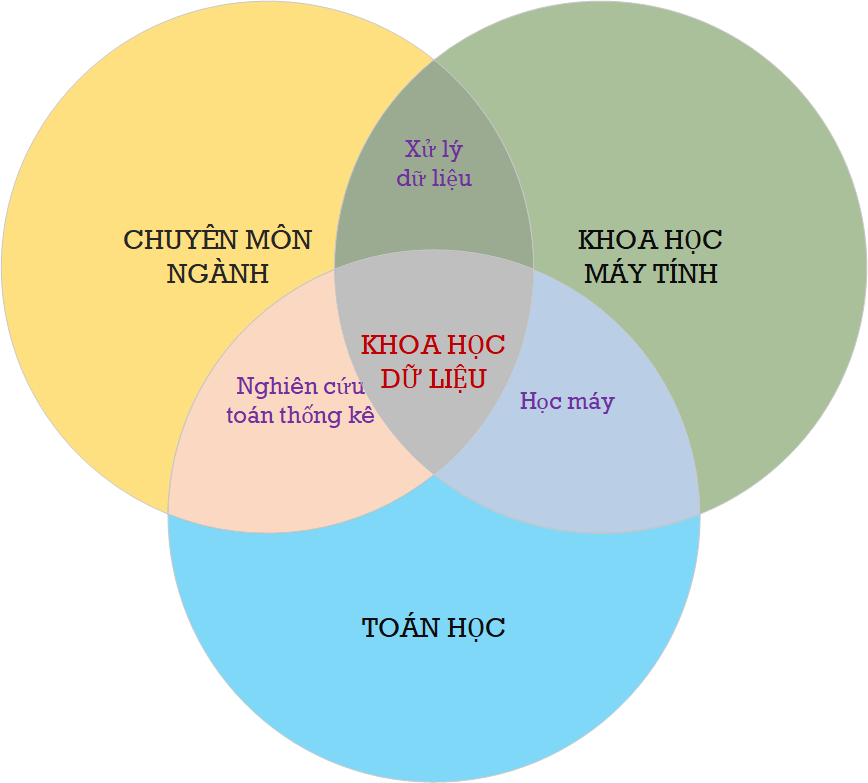
\includegraphics[width=8cm]{khoahocdulieu01}% This is a *.eps file
	\end{center}
	\caption{Giao thoa các mảng kiến thức - khoa học dữ liệu}\label{fig:khoahocdulieu01}
\end{figure}
\FloatBarrier

\FloatBarrier
\begin{figure}[h]
	\centering
	\begin{center}
		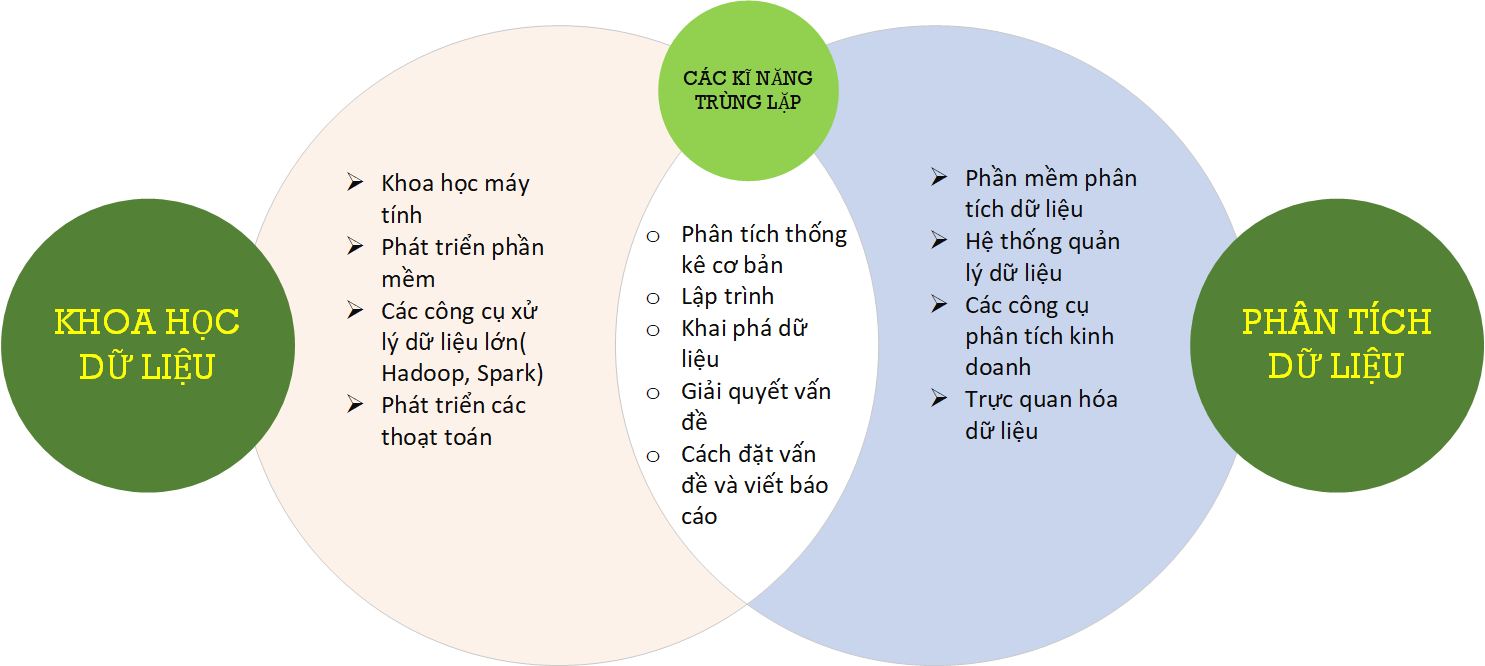
\includegraphics[width=\textwidth]{khoahocdulieu02}% This is a *.eps file
	\end{center}
	\caption{Các kĩ năng giao thoa - khoa học dữ liệu}\label{fig:khoahocdulieu02}
\end{figure}
\FloatBarrier

Một cái nhìn toàn diện về khoa học dữ liệu nhấn mạnh rằng "khoa học dữ liệu hơn là sự kết hợp của thống kê và khoa học máy tính" vì "nó yêu cầu đào tạo làm sao để tổng hợp và kết nối giữa các kĩ thuật thống kê và sức mạnh của máy tính trong một khung làm việc lớn hơn, giải quyết từng vấn đề một cũng như giải quyết các câu hỏi cụ thể trong từng lĩnh vực". Các nhà nghiên cứu cũng có cùng quan điểm cho rằng ngành khoa học dữ liệu đòi hỏi: (1) hiểu về bối cảnh của dữ liệu, (2) đánh giá các trách nhiệm liên quan đến việc sử dụng dữ liệu riêng tư và công khai; và (3) giao tiếp rõ ràng về những gì có thể và không thể được suy ra từ một bộ dữ liệu.

Các thành phần cốt lõi của khoa học dữ liệu là các phương pháp dựa trên học máy (Machine Learning - ML) để tìm kiếm các khuôn mẫu (pattern) trong dữ liệu và dựa vào đó để cung cấp thông tin về hiện tượng được mô tả bởi dữ liệu và các dự đoán liên quan đến các sự kiện trong tương lai. Trong học máy, mục tiêu là học/tạo ra một hàm (ánh xạ) mô tả và chứa đựng các dự liệu đầu vào (thường gọi là các biến giải thích - explanatory variable) với tham số đầu ra quan sát được (gọi là biến phản ứng - response variable). Một biểu diễn đơn giản hóa của thực tế được tạo ra cho mục đích này, gọi là mô hình, được sử dụng để ước tính phản ứng chưa biết cho các trường hợp mới dựa trên các biến giải thích quan sát được quan tâm, và quá trình này được gọi là suy luận hoặc đơn giản hơn là dự đoán.

Các mục tiêu của học máy thường được nhóm thành các nhiệm vụ mô tả và nhiệm vụ dự đoán. Các nhiệm vụ mô tả nhằm khám phá các mô hình có thể diễn giải được mô tả dữ liệu trong quá khứ, và các nhiệm vụ dự đoán là những nhiệm vụ mà mục tiêu là xác định các mô hình được quan sát trong dữ liệu huấn luyện để ước tính các dự đoán về các rủi ro và các kết quả khác trong tương lai. Các nhiệm vụ mô tả thường là không giám sát, có nghĩa là chỉ các biến giải thích được xem xét trong phân tích. Các mục tiêu mô tả phổ biến bao gồm phân cụm dữ liệu \citep{Albarakati2019, Gligorijevic2016}, khám phá mối liên hệ \citep{Gligorijevic2016a}, và phát hiện sự khác biệt so với hành vi bình thường, bao gồm phân tích giá trị cực đại, phát hiện giá trị ngoại vi và xác định các mô hình mới \citep{Tan2016}. Các nhiệm vụ dự đoán là giám sát, có nghĩa là chúng không chỉ yêu cầu các biến giải thích mà còn giá trị của biến phụ thuộc đang được dự đoán. Các ví dụ thực tế bao gồm đánh giá rủi ro và chẩn đoán bệnh \citep{Ghalwash2013}.

Có các phương pháp bán giám sát và tự đào tạo, trong đó dữ liệu huấn luyện bao gồm một số dữ liệu có nhãn và nhiều dữ liệu không có nhãn. 

Trong phân loại, các biến phản hồi được dự đoán là một lớp (ví dụ, một trong vài loại nhãn dữ liệu), hoặc trong trường hợp hồi quy, đó là một giá trị liên tục. Một trong những phương pháp thường được sử dụng cho phân loại là cây quyết định (decision tree). Thuật toán Hunt \citep{Tan2016}, một trong những phương pháp cây quyết định sớm nhất, đề xuất quy trình tổng quát của việc phân chia dữ liệu dựa trên giá trị của một thuộc tính duy nhất và tiếp tục đệ quy trên các tập con nếu lớp không đủ thuần khiết ở các tập con. Nhiều phương pháp đã được đề xuất để đo độ không thuần khiết của tập dữ liệu và xác định phân nhánh tiếp theo (ví dụ: entropy trong CART \citep{Breiman2017} hoặc chỉ số Gini trong ID3 \citep{Quinlan1986} và C4.5 \citep{Quinlan2014}), cũng như để tỉa cây, từ đó cải thiện khả năng tổng quát của mô hình. Cây quyết định dễ hiểu và không tốn kém nguồn lực để xây dựng và rất nhanh trong việc phân loại các trường hợp không rõ ràng. Chúng cũng khá bền với nhiễu và có thể xử lý các thuộc tính trùng lặp hoặc không liên quan, nhưng không tính đến sự tương tác giữa các thuộc tính. Một trong những hạn chế của cây quyết định là chúng yêu cầu tỉa, nếu không chúng sẽ trở nên quá lớn dẫn đến các vấn đề kĩ thuật như quá khớp (overfit). Giới hạn này được giải quyết thành công bằng Random Forests, được xây dựng như một tập hợp các cây quyết định không tương quan \citep{Breiman2001}. Tập hợp này được lấy cảm hứng từ phương pháp Bagging, một phương pháp tổng hợp dựa trên lấy mẫu bootstrap, được phát triển để giảm phương sai mà không làm tăng sai số \citep{Breiman1996}. Trong Random Forests, ý tưởng này được mở rộng hơn nữa bằng cách giới hạn mỗi nút chỉ xem xét một tập con ngẫu nhiên nhỏ của các thuộc tính. Giải pháp kết quả được chứng minh là chính xác hơn so với thuật toán AdaBoost.

Một kỹ thuật thay thế phổ biến có thể xử lý các tương tác giữa các biến giải thích là phân loại một trường hợp mới bằng cách tính khoảng cách đến k láng giềng gần nhất trong tập huấn luyện và dự đoán lớp dựa trên đa số hoặc đa số có trọng số của các láng giềng được xác định kết quả của chúng. Đây là một phương pháp học ít tốn kém vì mô hình không được xây dựng rõ ràng và thời gian suy luận cần thiết để phân loại một trường hợp mới khá lớn. Nó cũng yêu cầu so sánh mỗi điểm dữ liệu mới với mỗi điểm dữ liệu trong tập huấn luyện. Ngoài ra, kỹ thuật này không dễ sử dụng khi nhiều giá trị thuộc tính bị thiếu, vì trong những trường hợp như vậy, phương pháp dựa trên khoảng cách để xác định láng giềng gần nhất có thể không đáng tin cậy. Một số trong số những giới hạn này có thể được vượt qua bằng cách sử dụng nhánh mạng gần nhất (proximity graphs), trong đó các nút mạng được kết nối nếu các điều kiện hình học nhất định được đáp ứng. Trong một công thức như vậy, các thuật toán đồ thị hiệu quả khác nhau (ví dụ: cây khung nhỏ nhất và tam giác hóa) có thể được sử dụng để xác định láng giềng gần nhất và tương quan hơn.

Một phương pháp phân loại thay thế toán học nghiêm ngặt hơn là ước tính xác suất hậu nghiệm của lớp mục tiêu bằng cách sử dụng định lý Bayes. Một phương pháp khá đơn giản nhưng trơn tru và mạnh mẽ, được gọi là phương pháp Naive Bayes. Phương pháp này giả định rằng các giá trị thuộc tính độc lập có điều kiện với nhau, cho trước nhãn lớp $y$. Trong trường hợp như vậy, xác suất có điều kiện của lớp của tất cả các thuộc tính có thể được phân tách thành tích của xác suất có điều kiện của mỗi thuộc tính. Phương pháp này ngăn được nhiễu, giá trị bị thiếu và các thuộc tính không liên quan. Tuy nhiên, sự độc lập có điều kiện giữa các biến giải thích là một giả định mạnh mẽ không hợp lệ trong nhiều ứng dụng. Đối với các kịch bản như vậy, một lớp mô hình mạng lưới xác suất được gọi là Mạng tin cậy Bayesian đã được phát triển bằng cách mô hình hóa các phụ thuộc có điều kiện thông qua các mạng vô hướng và có hướng. Sự suy luận chính xác trên các mạng như vậy gọ là NP-hard \citep{Cooper1990}, do đó, các ứng dụng của chúng bị giới hạn cho số lượng thuộc tính nhỏ hơn hoặc cho các loại cấu trúc mạng lưới đặc biệt.

Một phương pháp phân loại theo xác xuất cũng khá hiệu quả là phương pháp hồi quy logistic. Khá nhiều ứng dụng sử dụng phương pháp này để dự đoán xác xuất mất điện liên quan đến thời tiết đã được triển khai. Điểm mạnh của phương pháp hồi quy logistic so với phương pháp láng giếng gần (k-nearest neighbour) là nó có thể giải quyết các vấn đề có nhiều chiều, bởi vì phương pháp này không dựa vào việc đo lường sự giống nhau giữa các điểm dữ liệu. Một lợi ích khác của phương pháp này là các tham số trọng lượng tương ứng với các thuộc tính riêng lẻ và do đó có tính giải thích khá dễ dàng. Tuy nhiên, sự hiện diện của một số lượng lớn các thuộc tính không liên quan là một thách thức đối với hồi quy logistic, và phương pháp này không áp dụng cho việc phân loại các trường hợp với giá trị rỗng, điều này có thể là một hạn chế lớn khi áp dụng trong thực tế với gói dữ liệu tồn tại số lượng lớn giá trị rỗng.

Mô hình hồi quy logistic có thể được xem như một trường hợp của mô hình tuyến tính tổng quát. Các mô hình mạnh mẽ khác trong danh mục này bao gồm Support Vector Machines (SVM) và Mạng neural đa tầng (Multilayer Neural Network - MNN). Trong phương pháp SVM, vấn đề tối ưu hóa được định hình như tìm kiếm ranh giới lớn nhất phân tách siêu mặt phẳng cho một khu vực lớn tồn tại ở mỗi bên của ranh giới quyết định \citep{Cortes1995}. Điều này được định hình như một vấn đề lập trình phi tuyến tính bị ràng buộc được biểu thị dưới dạng một hàm của các hệ số của siêu mặt phẳng phân tách, được giải quyết bằng phương pháp bội số Lagrange. Đối với phân loại phi tuyến tính, dữ liệu được chuyển đổi một cách ngầm định thành không gian đa chiều, nơi vấn đề có thể được phân tách theo dạng tuyến tính. Điều này được đạt được bằng cách sử dụng thủ thuật Kernel, để giảm bớt vấn đề thành tình huống phân loại tuyến tính. Sử dụng các Kernel được chọn cẩn thận (Gaussian, đa thức, hoặc sigmoid) cho phép xấp xỉ các ranh giới quyết định tùy ý. Các lợi ích chính của phương pháp SVM là nó chống lại nhiễu và giảm thiểu overfitting trong khi tìm kiếm giá trị nhỏ nhất toàn cục của hàm mục tiêu. Tuy nhiên, chi phí tính toán của SVM là cao, và vẫn là một thách thức để sử dụng mô hình này khi các biến mô tả bị thiếu một phần trong dữ liệu quan sát.

Mạng nơ-ron tiến thẳng đa tầng (Multiplayer Feed-Forward Neural Network - FNN) cũng được sử dụng thành công cho phân loại trong nhiều ứng dụng khác nhau \citep{Zhang2000}. Ví dụ như việc áp dụng thành công trong việc huấn luyện FNN để phân biệt giữa dòng vào từ biến áp và dòng lỗi \citep{Perez1994}. Mô hình này có ít nhất một lớp đơn vị ẩn, mỗi lớp tính toán một hàm phi tuyến mượt và khả vi của tổng đầu vào có trọng số (ví dụ, hàm sigmoid). Trong mô hình này, vấn đề cập nhật các tham số khi phát hiện lỗi ở đầu ra thường được giải quyết bằng cách truyền ngược lỗi từ đầu ra về các lớp trước đó. Trong quá trình này, lỗi của một nút trong lớp ẩn được ước tính dưới dạng một hàm của các ước tính lỗi và trọng số trong các nút trong lớp trước đó, và giá trị này được sử dụng để cập nhật trọng số của nút ẩn này bằng cách tính toán độ dốc lỗi đối với các trọng số trong nút \citep{Werbos1994}. FNN có thể xấp xỉ các hàm tùy ý, và do đó mạnh mẽ hơn SVM. Tuy nhiên, khi thiết kế một mạng, overfitting phải được giải quyết cẩn thận. Ngoài ra, nhiễu trong dữ liệu có thể gây ra vấn đề huấn luyện, vì mô hình có thể hội tụ đến một cực tiểu cục bộ, và quá trình huấn luyện có thể yêu cầu một thời gian dài, do đó giới hạn tới việc triển khai cho các ứng dụng thực tế. Vấn đề khác với phương pháp FNN truyền thống là học các mạng sâu rất khó, do tác động kết hợp của việc bão hòa hàm kích hoạt sigmoid khi truyền ngược các lỗi nhỏ, dẫn đến sự hội tụ rất chậm. Tiến bộ lớn đã được đạt trong việc giải quyết vấn đề này, được gọi là vấn đề gradient biến mất (Vanishing Gradient Problems), trong những năm gần đây. Điều này, cùng với tiến bộ trong cơ sở hạ tầng tính toán phân tán dựa trên GPU và sự có sẵn của các tập dữ liệu rất lớn, đã cho phép phát triển các mạng nơ-ron sâu hiệu quả, vượt trội hơn rất nhiều so với tất cả các phương pháp truyền thống, bao gồm thị giác máy tính (Computer Vision), xử lý ngôn ngữ tự nhiên, phát âm. trong những năm gần đây, nhiều kiến trúc học sâu đã được đề xuất và phát triển để xử lý dữ liệu với nhiều thuộc tính khác nhau, tiêu biểu trong số đó là phương pháp mạng nơ-ron tích chập (Convolutional Neural Network) áp dụng để xử lý dữ liệu toàn mạng lưới điện (ví dụ như các dữ liệu về ảnh) và mạng nơ-ron hồi quy cho chuỗi dữ liệu thời gian \citep{Werbos1994, LeCun2015}.

%Đối với các hệ thống điện, dữ liệu thường được quan sát và thu thập cả về mặt không gian và thời gian, do đó, các phương pháp hồi quy tiên tiến dựa trên cấu trúc  mạng lưới thường được áp dụng hơn để khai thác các sự phụ thuộc về mặt trúc (Ví dụ như sử dụng mô hình học máy được tích hợp phương pháp Bayes với trường ngẫu nhiên để đánh giá rủi do liên quan đến sự hủy hoại lớp cách điện khi thiết bị được đặt vào môi trường có nguy cơ liên quan đến thời tiết trong một mạng lưới). Các nghiên cứu về học sâu đều đưa ra kết luận rằng các ứng dụng, bao gồm hồi quy cấu trúc, có thể được hưởng lợi từ việc học các biểu diễn tiềm ẩn cho dữ liệu đầu vào. Trong một số nghiên cứu, việc học biểu diễn cho các trạm hệ thống điện, dựa trên sự gần nhau về không gian của chúng, đã chứng minh là rất có lợi cho việc dự đoán các lỗi liên quan đến cung cấp điện và ước tính xác suất lỗi đó. 

%Trong một phương pháp như vậy, các nút của đồ thị được nhúng trong không gian chiều thấp hơn, nơi các phương pháp học máy tiêu chuẩn có thể được áp dụng dễ dàng hơn. Các thuật toán nhúng nhằm giữ cấu trúc đồ thị và đơn giản hóa các mô hình học bằng cách di chuyển khỏi các biểu diễn đồ thị. Một lợi thế của việc sử dụng các phương pháp này là chúng có thể tiết lộ các phụ thuộc không gian phức tạp hơn có chứa một số tương tác xa hơn ngoài tác động của khu vực lân cận.

%Quá trình nhúng nút đại diện cho đồ thị ban đầu trong một không gian đặc trưng mới, mô tả tốt nhất các mối quan hệ không gian của các nút trong đồ thị ban đầu. Đặc điểm này của quá trình nhúng nút nhằm bắt giữ các mối quan hệ cần thiết của cấu trúc đồ thị ban đầu trong khi đơn giản hóa biểu diễn thành một danh sách các vector đặc trưng chiều thấp hơn.

%Có nhiều thuật toán để thu được nhúng như vậy; Hai thuật toán thường được sử dụng là DeepWalk [95] và Node2Vec [96]. Cả hai thuật toán đều dựa trên thông tin cộng đồng được thu được bằng các bước đi ngẫu nhiên, được sử dụng để học các biểu diễn không gian tiềm ẩn. Ngoài ra, DeepWalk có thể thực hiện khám phá cục bộ một cách hiệu quả và có thể chứa đựng các thay đổi nhỏ trong cấu trúc đồ thị mà không cần tính toán toàn cầu lại. Node2Vec là một khung công cụ thuật toán hóa mà tổng quát hóa quá trình DeepWalk để cung cấp một khái niệm linh hoạt về khu vực lân cận của một nút, cho phép học các biểu diễn phong phú hơn bằng cách khám phá hiệu quả các khu vực lân cận đa dạng. Giải pháp này đã được sử dụng thành công để phát triển một phương pháp mới cho dự báo bức xạ mặt trời, dựa trên các nhúng không gian và thời gian sử dụng mô hình Node2Vec cho dữ liệu đồ thị [97]. Phương pháp này đơn giản hóa các mô hình học bằng cách di chuyển khỏi các đồ thị phức tạp. Mô hình được phát triển cho các dự báo từ 3 đến 12 giờ. Mô hình đã dự đoán bức xạ mặt trời với độ chính xác rất cao vào mùa hè, khi có nhiều ngày trời quang đãng. Trong những tháng mùa đông, độ chính xác có một chút giảm, nhưng vẫn rất cao và vẫn mạnh mẽ ngay cả khi dữ liệu quan sát bị thiếu về mặt không gian và thời gian.


\subsection{Khía Cạnh Kĩ Thuật}
%Trong khi phân tích dữ liệu lớn dựa trên nền tảng khoa học dữ liệu mạnh mẽ, cũng có một số khía cạnh quan trọng khác để các phương pháp đó được sử dụng trong thực tế. 
Có một thực tế đã được nhiều chuyên gia và nhà nghiên cứu tổng kết là, thực tế làm các công việc phân tích và mô hình liên quan đến xử lý dữ liệu lớn thường chỉ chiếm khoảng 10\% tổng số công việc (số giờ, tài nguyên) liên quan đến cả quá trình xử lý dữ liệu. Có đến 90\% công việc lại trực tiếp liên quan đến thiết lập quy trình làm việc, quản lý dữ liệu (và lưu trữ) cũng như các khía cạnh tính toán. Do đó, việc quan sát và tập trung nguồn lực vào một số khía cạnh liên quan đến kỹ thuật trong phân tích dữ liệu lớn là rất quan trọng. Chúng đã được xác định là các thách thức chính cho sự thành công của phân tích dữ liệu lớn \citep{Wickham2023}.

Ở trung tâm của khái niệm phân tích dữ liệu lớn cơ bản là việc chúng ta cho rằng dữ liệu cần được xử lý là "lớn". Để định nghĩa đúng dữ liệu lớn và các tính năng cần thiết của nó, người đọc được giới thiệu đến \citep{DeMauro2016}. Các ví dụ điển hình liên quan đến việc thu thập dữ liệu PMU, cũng như dữ liệu có độ phân giải cao ở mức tài sản, (ví dụ, từ các tuabin gió, bộ biến tần điện từ (PV), công tơ thông minh, v.v.). Tốc độ thu thập dữ liệu này ở các thang thời gian từ giây đến phút, và đồng thời ở nhiều vị trí địa lý khác nhau, trong khi cũng bao gồm nhiều loại biến số khác nhau. Nói chung, các dữ liệu như vậy trong lưới điện bao gồm các dữ liệu đo lường điểm, hình ảnh và có thể là văn bản. Một số khía cạnh của dữ liệu lớn này cho các hệ thống điện, từ thách thức đến ứng dụng, đã được \cite{Arghandeh2017} đề cập gần đây .

Việc đảm bảo tính của giao tiếp dữ liệu, đảm bảo tính toàn vẹn của dữ liệu, cũng như đảm bảo chất lượng dữ liệu, là các bước cần thiết và quan trọng trước khi tiến hành thiết kế và triển khai một giải pháp dựa trên dữ liệu \citep{Cai2015}. Ngược lại, những khía cạnh liên quan đến tính sẵn có và chất lượng dữ liệu đã được xem xét trong một thời gian khá lâu bởi cộng đồng khoa học máy tính \citep{Batini2009}. Tiếp theo đó là việc làm sạch dữ liệu và sửa đổi các bộ dữ liệu có liên quan, mặc dù người ta nên nhận thức rằng những hành động này thực sự có thể ảnh hưởng đến thông tin ban đầu trong các bộ dữ liệu. Đối với các ứng dụng trong các thị trường điện liên quan đến năng lượng tái tạo, một vấn đề khá truyền thống liên quan đến ví dụ là điền vào các khoảng trống trong chuỗi thời gian, tức là có thể có các khoảng thời gian mà dữ liệu không có sẵn, do các lỗi trong việc đăng nhập, lưu trữ hoặc truyền dữ liệu. Để điền vào những khoảng trống này, đã có nhiều nhiều phương pháp được đưa ra như việc  tận dụng dữ liệu xung quanh khoảng thời gian đó, hay dữ liệu với phụ thuộc không gian thời gian (đặc biệt liên quan đến việc tạo ra năng lượng tái tạo dựa trên thời tiết), tính sẵn có của dữ liệu ở các mức tổng hợp khác nhau, cũng như mối quan hệ vật lý giữa các biến số quan tâm.

Ngoài những khía cạnh liên quan đến dữ liệu, các phương pháp dựa trên dữ liệu được sử dụng trên các tập dữ liệu lớn đòi hỏi năng lực tính toán đáng kể để giải quyết các vấn đề mô phỏng và tối ưu hóa liên quan. Chẳng hạn như việc sử dụng phương pháp tính toán hiệu năng cao  (High Performance Computing - HPC) cho việc tập trung hóa xử lý. Phương pháp HPC ngày càng trở nên phổ biến trong các ứng dụng phân tích lưới điện và thị trường điện \citep{Khaitan2012}. %Việc giải quyết các vấn đề quy mô lớn với HPC sẽ liên quan đến một số kỹ thuật phân rã, cũng trở nên phổ biến trong các vấn đề vận hành, thị trường và kế hoạch hệ thống điện [108]. Tuy nhiên, cũng có thể có một số ứng dụng mà điều này không phải là khả thi hoặc không muốn tập trung dữ liệu. Trong trường hợp đó, các phương pháp tương tự có thể được sử dụng để giải quyết các vấn đề này theo cách phi tập trung, tuy nhiên, có thể phải chịu gánh nặng giao tiếp tăng do tính chất lặp lại của các phương pháp tối ưu hóa phân tán. Những ví dụ đáng chú ý bao gồm các vấn đề luồng công suất tối ưu [109] và học phân tán cho dự báo năng lượng tái tạo [110]. Có lẽ trong tương lai, các thiết lập liên quan sẽ không được tập trung hoàn toàn hoặc phi tập trung hoàn toàn và sẽ phụ thuộc vào tính toán đám mây, fog và edge computing [111].

Phân tích dữ liệu lớn cần được đặt trong khung quản lý tổng thể để giải quyết một hay nhiều vấn đề cụ thể. Trong thực tế, đó chỉ là một công cụ bổ sung để hỗ trợ hoạt động và ra quyết định. Do đó, trước khi đầu tư vào các thiết lập dữ liệu lớn cụ thể và các công cụ phân tích, vấn đề và phương pháp giải quyết vấn đề liên quan cần được xác định rõ ràng. Ví dụ, nếu các dự báo được sử dụng để hỗ trợ ra quyết định, loại dự báo (ví dụ, xác định hoặc xác suất) và các sản phẩm dự báo (độ phân giải, chuẩn hóa, vv.) nên được quyết định dựa trên vấn đề quyết định cụ thể. Ngoài ra, khi chuyển từ dữ liệu sang dạng thứ cấp để phục vụ phân tích, thường nên tạo ra một lớp trích xuất/chú giải đúng loại và mức thông tin từ dữ liệu thô để về sau dễ liên hệ. %Điều này có thể được thực hiện dựa trên các phương pháp liên quan đến lọc và làm mịn, kỹ thuật kỹ thuật đặc trưng, vv. Một ví dụ điển hình sẽ là phát hiện sự kiện dựa trên các luồng dữ liệu, sau đó được sử dụng làm đầu vào cho một số vấn đề phân tích khác.

Các yêu cầu bổ sung có thể mang lại một cấp độ phức tạp khác cho phân tích dữ liệu lớn. Yêu cầu quan trọng liên quan đến dữ liệu chính nó (và các luồng dữ liệu liên quan) là cách xử lý an ninh mạng và quyền riêng tư trong lưới điện. Hiện nay, an ninh mạng đại diện cho một thành phần quan trọng của hệ thống năng lượng phân phối trong tương lai, mà trên đó phân tích dữ liệu lớn có thể được thực hiện \citep{Li2017}. Do đó, công tác thiết lập cho việc phân tích dữ liệu lớn, cũng như các công cụ được sử dụng, cần phải mạnh mẽ để có thể chịu đựng được việc loại bỏ các dữ liệu quan trọng hoặc làm giả dữ liệu. Ngoài ra, quyền riêng tư dữ liệu đang trở thành mối quan tâm ngày càng tăng vì nếu dữ liệu đang được thu thập được chia sẻ, có thể suy ra thông tin các nhân về các tài sản hoặc người tiêu dùng cụ thể. Mối quan tâm về quyền riêng tư đặc biệt hiện nay khi các công tơ thông minh được triển khai rộng rãi, cho phép một số người có thể có thông tin về thói quen tiêu dùng của người khách hàng để tiến hành các hoạt động tiếp thị và tội phạm. %Yêu cầu chính khác liên quan đến nhu cầu có các mô hình và kết quả có thể giải thích được. Điều này đã kích hoạt một lĩnh vực nghiên cứu mới liên quan đến việc học máy có thể giải thích và học máy dựa trên vật lý.

\subsection{Khung Đưa ra Quyết Định}
Việc sử dụng phân tích dữ liệu lớn tất yếu sẽ dẫn đến việc nâng cao khả năng ra quyết định. Do đó, việc trực quan hóa trong toàn bộ quá trình xử lý nên được đặc biệt quan tâm vì các nhà quản lý và điều hành thường đưa ra các quyết định dựa trên các con số và bảng biểu hay đồ thị được trực quan hóa.

Trong trong những vấn đề giành được sự quan tấm lớn hiện nay, không những chỉ trong ngành điện, mà còn trong công tác quản lý hạ tầng nói chung đó là việc quản lý rủi do. Trong công tác quản lý rủi do, ngoài việc đưa ra các mức rủi do mang tính chất định tính, các nhà quản lý cũng cần phải yêu cầu các kĩ sư và nhà phân tích đưa ra các con số định lượng và trực quan hóa các nguy cơ gây ra rủi do, mức độ tổn thương mạng lưới và rủi do cho từng bộ phân và khu vực trên toàn mạng lưới (Hình \ref{fig:2}). Như ví dụ ở Hình \ref{fig:2}, một bản đồ rủi do được thiết lập dựa trên việc tích hợp của hai bản đồ nền tảng là bản đồ nguy cơ và bản đồ tổn thương.

\FloatBarrier
\begin{figure}[h]
	\centering
	\begin{center}
		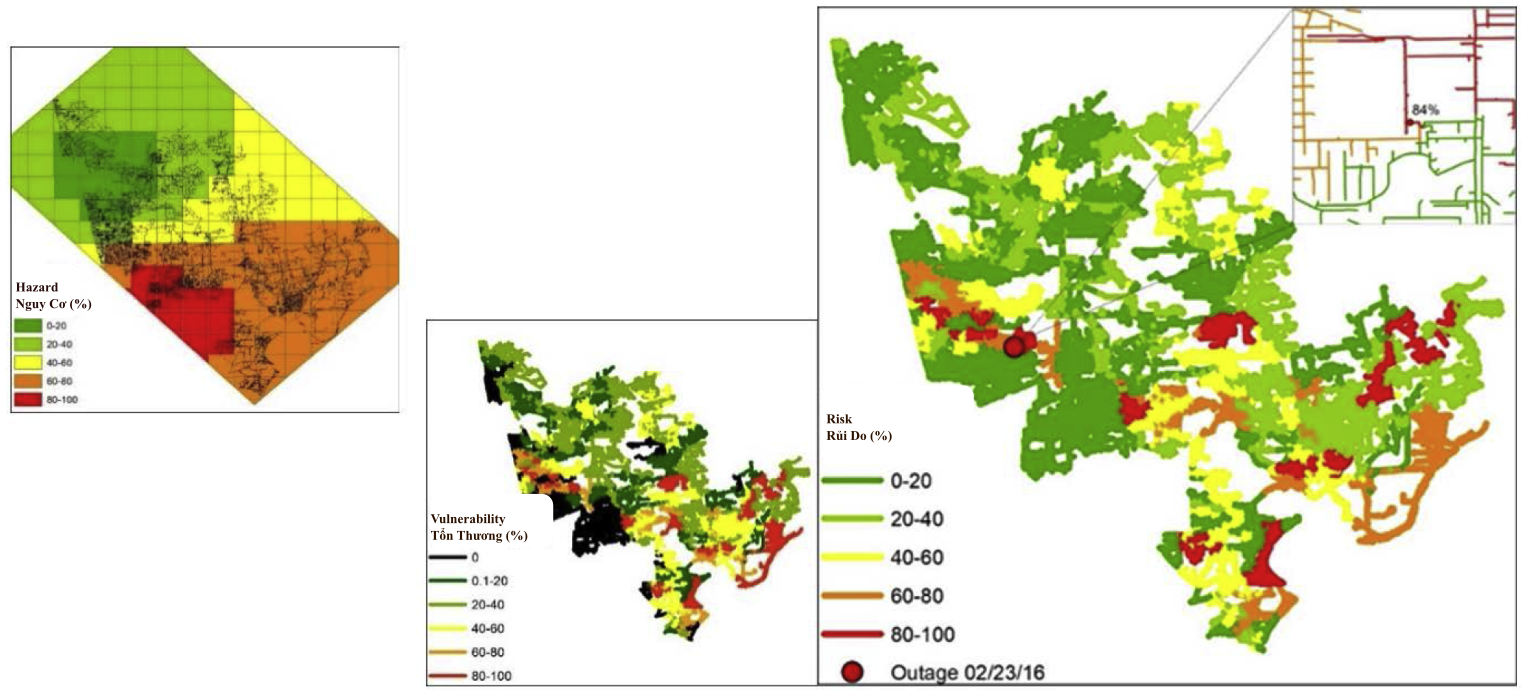
\includegraphics[width=15cm]{ruido}% This is a *.eps file
	\end{center}
	\caption{Bản đồ thể hiện nguy cơ, sự tổn thương, và rủi do của mạng lưới}\label{fig:2}
\end{figure}
\FloatBarrier

Như chúng ta đã thấy, việc đánh giá rủi do là khá phức tạp, đặc biệt là trên phương diện mạng lưới. Do đó, để tính toán được một cách có hệ thống và đạt được một mức độ chính xác nhất định, chúng ta cần phải xây dựng một khung công việc (framewwork) hay một dòng chảy công việc (work flow) nền tảng. Các khung công việc hay dòng chảy công việc này cần được thiết lập cho từng cấp độ khác nhau. Ở phạm vi quốc tế, ví dụ chúng ta có thể thấy đó là khung công việc cho đánh giá rủi do được đưa ra bởi Văn phòng Cứu trợ Khẩn cấp của Liên Hợp Quốc (UNDRO), hay Văn phòng Liên Hợp Quốc về Giảm thiểu Rủi ro Thiên tai (UNISDR). Ở mức độ quốc gia, chúng ta có thể lấy ví dụ về các tiêu chuẩn được đưa ra bởi Cơ quan Quản lý Khẩn cấp Liên bang (FEMA) của Hoa Kỳ.%., vì trọng tâm chính là ảnh hưởng liên quan đến khí hậu đến cơ sở hạ tầng, xã hội và môi trường. Điều này giới thiệu Trạng thái Rủi ro (SoR) như sau:

Rủi được thể hiện qua công thức tính toán đơn giản sau.

\begin{equation}\label{math01}
	\textbf{R}isk = \textbf{H}azard \times \textbf{V}ulnerability \times \textbf{C}onsequences
\end{equation}

Nguy cơ (H) và sự tổn thương (V) có thể được xác định bằng xác xuất. Nguy cơ có thể được tính toán dựa trên xác xuất của một sự kiện nào đó (chẳng hạn như động đất, lũ lụt, mưa lớn) xảy ra với mức độ hay độ mạnh khác nhau (thường gọi là Intensity). Tổn thương (V) liên quan trực tiếp tới yếu tố bản thân của thiết bị tài sản, như xự xuống cấp hay các thông số thiết kế và độ mạnh của nguy cơ. Ở nhiều góc độ khác, tổn thương còn liên quan đến các yêu tố quản lý và sự sẵn sàng của doanh nghiệp trước các sự cố và hiện tượng bất thường.

Thiệt hại (C) cần phải được tính toán cụ thể và thường được đo bởi đơn vị tiền tệ. Ở đây, thiệt hại nên được hiểu theo nghĩa rộng, tức là không chỉ dừng lại ở việc đo lường thiệt hại cho doanh nghiệp, mà còn phải đo lường thiệt hai cho cộng đồng và cho môi trường. Để tính toán và lượng hóa được thiệt hại cần phải xây dựng một hệ thống hay cấu trúc thông xuốt để loại trừ cách tính trùng lặp (thường được hiểu là thiết lập một Impact Hierachy). Một số phương pháp tiêu biểu có thể được áp dụng để tính toán H, V, và C là phương pháp Fault-Tree Analysis (FTA), hay còn gọi là phân tích lỗi theo dạng cây và phương pháp Event Tree Analysis (ETA) hay còn gọi là phân tích sự kiện theo dạng cây.

%trong đó P(T) là Nguy cơ hoặc xác suất của một mức độ mối đe dọa cụ thể (T); u(C) là Tổn thất (xã hội, kinh tế hoặc môi trường) liên quan đến mức độ Hậu quả (C), liên quan đến mức độ mối đe dọa (T); và P(C|T) là Tính dễ tổn thương hoặc xác suất của việc trải qua mức độ hậu quả (C) được xác định dựa trên mức độ mối đe dọa (T). Đơn vị rủi ro được biểu thị trong đơn vị của các tổn thất.

Việc tính toán rủi do là quan trọng, nhưng cũng chỉ là một bước nếu đặt trong một mô hình toán tối ưu (Optimization Model) khi mà các nhà quản lý cần quan tâm đến nguồn lực nội tại cũng như các khó khăn phải đối mặt (Constraints). Do đó, sau khi tính toán được rủi do, cần xây dựng mô hình tối ưu với một hàm mục tiêu cụ thể và các giàng buộc đi kèm. Hình \ref{fig:3} mô tả khái quan một khung làm việc cho ví dụ về dự báo mất điện mạng lưới gây ra bởi thời tiết.

%Trong bối cảnh này, quyết định liên quan đến quá trình tối ưu hóa, trong đó hàm mục tiêu và ràng buộc nhằm mục đích hành động giảm thiểu được xác định. Một khung quyết định rộng hơn cho các ví dụ về dự báo mất điện đã được hiển thị trong Hình \ref{fig:3}.
\FloatBarrier
\begin{figure}[h]
	\centering
	\begin{center}
		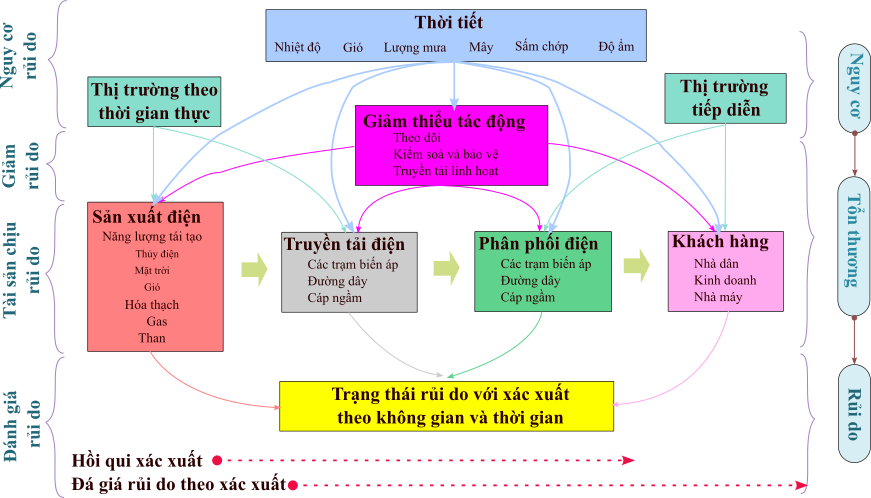
\includegraphics[width=15cm]{decisionmaking-risk}% This is a *.eps file
	\end{center}
	\caption{Khung ra quyết định cho việc đánh giá rủi do}\label{fig:3}
\end{figure}
\FloatBarrier

\section{Ứng Dụng}
\subsection{Quản Lý tài Sản Cơ Sở Hạ Tầng và Sự Cố Mất Điện}
Tại các thị trường có sự cạnh tranh về điện, tư nhân hóa và các yêu cầu kỹ thuật hoặc quy định bắt buộc các công ty điện phải tối ưu hóa công tác quản lý và vận hành. Trong thực tế hoạt động của công ty điện, quản lý tài sản và quản lý sự cố mất điện được xử lý bởi các nhóm khác nhau và thường được đề cập trong việc lập kế hoạch từ ngắn hạn đến dài hạn. Việc quản lý tài sản và quản lý sự cố mất điện có mối tương quan với nhau và chính vì thế việc sử dụng dữ liệu của cả hai nhóm này trên cùng một hệ thống và nền tảng phân tích sẽ là một trong những ưu tiên nên được đầu tư và quan tâm thích đáng.

Các công ty và doanh nghiệp điện lực thường chú trọng nhiều hơn đến việc quản lý sự cố mất điện chứ chưa có đầu tư đích đáng vào quản lý tài sản. Ở các nước phát triển, có một thực tế là việc quản lý tài sản nói chung và ngành điện nói riêng cũng chỉ được quan tâm trong vòng 15 năm trở lại đây. Đã có khá nhiều phần mềm quản lý tài sản, gọi chung là CMMS (Computerized Maintenance and Management Systems) đã được phát triển và đưa vào sử dụng. Nhưng ở các nước đang phát triển, trong đó có Việt Nam, quản lý tài sản là một khái niệm tương đối mới và chưa có một trường đại học nào đào tạo về ngành này. 

Về cơ bản, theo tác giả, quản lý tài sản có thể được định nghĩa là "\textbf{Tối ưu hóa việc phân bổ nguồn tài nguyên có hạn cho công tác làm mới hay duy tu vả bảo dưỡng các thiết bị và hệ thống sẵn có. Việc tối ưu hóa phải được tính đến lợi ích và ảnh hưởng của doanh nghiệp cũng như của các bên liên quan và môi trường}". Hình \ref{fig:asset} mô tả các qui trình và công đoạn cần thiết cấu thành lên một hệ thống quản lý tài sản hoàn chỉnh.

\FloatBarrier
\begin{figure}[h]
	\centering
	\begin{center}
		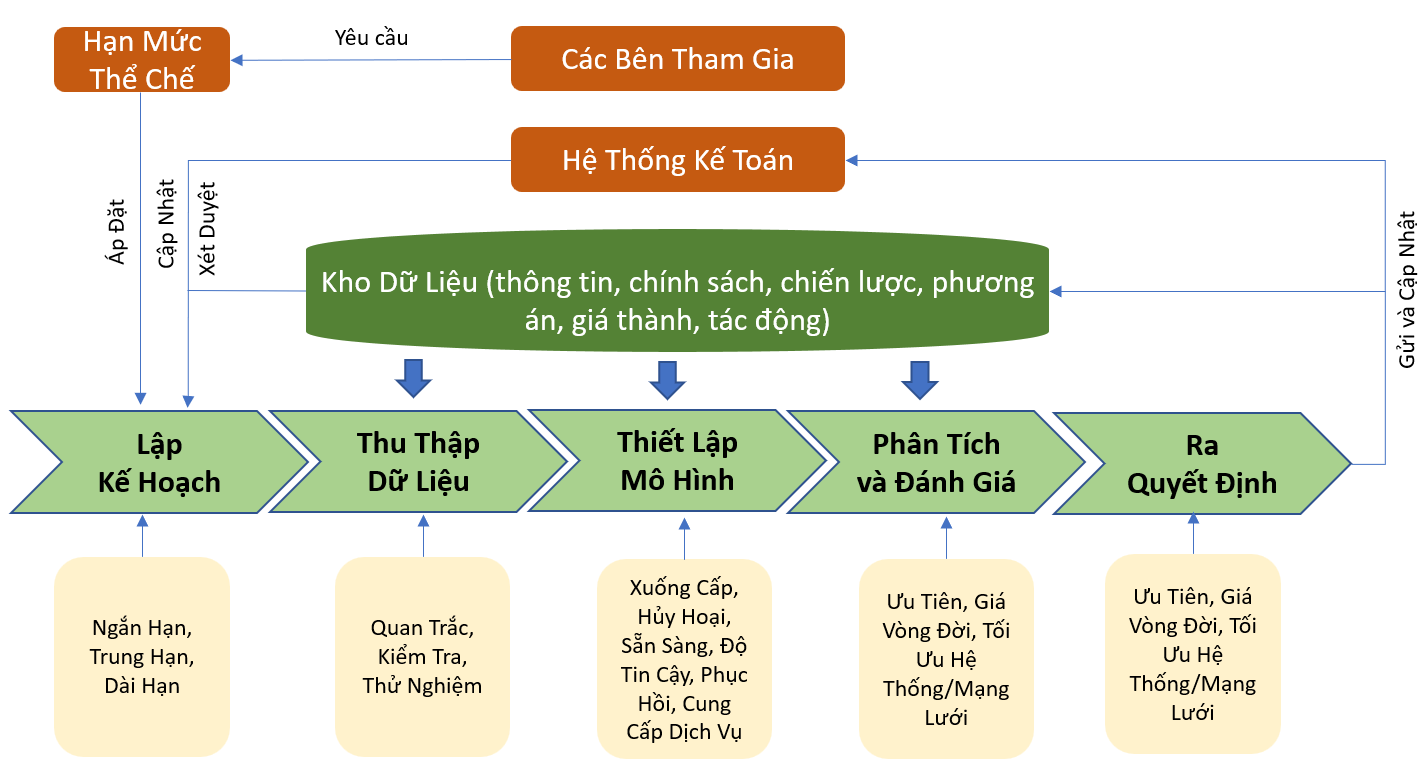
\includegraphics[width=14cm]{assetmanagement}% This is a *.eps file
	\end{center}
	\caption{Qui trình và công đoạn trong quản lý tài sản hạ tầng}\label{fig:asset}
\end{figure}
\FloatBarrier

%Chúng tôi đã giữ cuộc thảo luận về các vấn đề có vẻ không liên quan này cùng với nhau để nhấn mạnh sự tương quan chặt chẽ giữa chúng về việc sử dụng dữ liệu, vì quản lý gián đoạn có thể sử dụng cùng dữ liệu với quản lý tài sản và ngược lại vì tình trạng cơ sở của tài sản điều khiển cả hai ứng dụng:

%\begin{enumerate}
\subsubsection{Phân Loại Tài Sản} 

Quản lý tài sản trong các hệ thống điện có thể được phân loại rộng rãi thành bốn loại chính dựa trên các thời gian thời gian thực, ngắn hạn, trung hạn và dài hạn. 

Quản lý tài sản thời gian thực chủ yếu bao gồm các nguyên tắc bền vững của hệ thống điện chính và xử lý các sự cố gián đoạn không đáng kể của thiết bị hệ thống điện và sự cố gián đoạn lưới điện. Bằng cách cải thiện nhận thức tình hình, các nhà điều hành lưới điện có thể giám sát và kiểm soát hệ thống một cách hiệu quả. Quản lý tài sản ngắn hạn cố gắng tối đa hóa tỷ lệ lợi nhuận liên quan đến đầu tư tài sản. Giá trị chủ yếu phụ thuộc vào giá thị trường không chắc chắn thông qua việc điều chỉnh và tác động vào thị trường. Đánh giá rủi ro thị trường là một yếu tố quan trọng và phân phối doanh thu/lợi nhuận được đạt thông qua phân tích tính lợi nhuận. Lập lịch bảo trì tối ưu thuộc quản lý tài sản trung hạn. Nó hướng dẫn kế hoạch bảo trì đến các mục tiêu mong muốn của toàn hệ thống một cách đầy đủ.

Các nỗ lực được tập trung vào tối ưu hóa phân bổ tài nguyên tài chính hạn chế ở những nơi và thời điểm cần thiết để quản lý gián đoạn tối ưu mà không đánh đổi tính đáng tin cậy của hệ thống. Sử dụng rộng rãi các công nghệ cảm biến thông minh và giám sát để đánh giá tình trạng làm việc và độ tin cậy của thiết bị và hệ thống theo thời gian và tối ưu hóa các kế hoạch bảo trì tương ứng. Đầu tư vào kế hoạch mở rộng hệ thống điện, cũng như triển khai rộng rãi các nguồn điện phân tán, thuộc phạm vi của quản lý tài sản dài hạn, trong đó các nhà đầu tư, các đối thủ cạnh tranh và các bên liên quan khác được mời tham gia vào các kế hoạch kinh tế trong tương lai.

%\end{enumerate}

\subsubsection{Tác Động của Thời Tiết và Sự Cố Mất Điện}
Tác động của thời tiết đối dẫn đến sự cố mất điện và gián đoạn trong hệ thống điện có thể được phân loại thành trực tiếp và gián tiếp:

\begin{itemize}
\item Tác động trực tiếp đối với tài sản hạ tầng điện: Loại tác động này bao gồm tất cả các tình huống khi điều kiện thời tiết nghiêm trọng trực tiếp gây ra sự cố với tài sản. Ví dụ như sét đánh vào thiết bị, tác động của gió khiến cho cây hoặc cành cây chạm vào đường dây, v.v. Những sự cố này được đánh dấu là sự cố do thời tiết gây ra.

\item Tác động gián tiếp đối với tài sản hạ tầng điện: Loại tác động này xảy ra khi thời tiết tạo ra một tình huống trong mạng lưới mà gián tiếp gây ra sự cố của thiết bị. Các ví dụ bao gồm: điều kiện thời tiết nóng làm tăng nhu cầu, gây quá tải cho đường dây dẫn đến giảm độ cao của đường dây, tăng nguy cơ sự cố do tiếp xúc với cây, thiết bị tiếp xúc với tác động của thời tiết trong dài hạn dẫn đến xuống cấp và giảm khả năng cung ứng dịch vụ, v.v. Những loại gián đoạn này được đánh dấu là lỗi thiết bị.

\end{itemize}

Ngoài hai khái niệm trên, thực tế là chúng ta có thể chia sự xuống cấp của thiết bị theo hai xu hướng: (1) Xuống cấp theo thời gian và có thể quan sát được (Manifest Deterioration) và (2) xuống cấp bất ngờ hay đột ngột (Latent/Sudden) do các nguyên nhân như thiên tai.

\subsubsection{Cơ Bản về Quản Lý Sự Cố Mất Điện}

Khả năng theo dõi đồng thời nhiều mối đe dọa do thời tiết gây ra và đánh giá các tác động và thiệt hại đến tài sản ngành điện hay các sở hạ tầng (hạ tầng giao thông) liên quan đến việc hỗ trợ cho ngành điện là rất quan trọng. Đơn giản bời vì, lưới điện được phân bổ trên các vùng rộng lớn với các nhà máy phát điện thường đặt ở những vùng xa xôi. Tiêu thụ lớn ở các khu đô thị có nghĩa là lưới truyền tải phải đưa điện từ các nhà máy phát điện ở xa đến các trung tâm tiêu thụ và hệ thống phân phối phải cung cấp các đường dẫn tiện ích cho từng khách hàng. Để đạt được điều này, lưới phải trải qua các trạng thái hoạt động khác nhau (Hình \ref{fig:grid}). Bằng cách kết hợp quản lý tài sản và quản lý sự cố mất điện, chúng ta có thể xử lý và giảm thiểu các tác động gây thiệt hại một cách hiệu quả nhất.

\FloatBarrier
\begin{figure}[h]
	\centering
	\begin{center}
		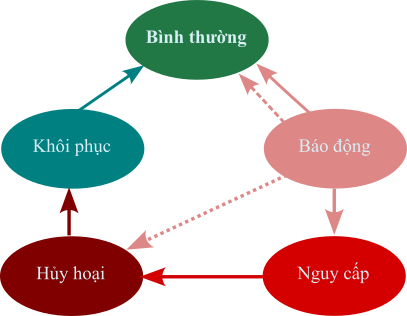
\includegraphics[width=6cm]{electricgridstates}% This is a *.eps file
	\end{center}
	\caption{Các trạng thái của lưới điện}\label{fig:grid}
\end{figure}
\FloatBarrier

\subsubsection{Tiên Đoán Mất Điện trên Mạng Lưới Truyền Tải}
Kiến thức từ dữ liệu thu thập trong quá khứ có thể được sử dụng để dự đoán những sự cố mất điện trên lưới điện liên quan đến thời tiết trong vòng 1-3 giờ trước. Các biến liên quan đến không gian được thêm vào bộ dữ liệu để tính toán được mối liên hệ tương hỗ giữa các sự kiện và các nút trên mạng lưới. Chương trình Hệ thống Quan sát Bề Mặt Tự Động (ASOS) được sử dụng để thu thập các đo lường thời tiết lịch sử cho các tham số sau: Hướng gió [độ], Tốc độ gió [km/h], Gió giật [m/s], Nhiệt độ [C], Điểm sương [F], Độ ẩm tương đối [\%], Áp suất [mb], Lượng mưa/giờ [mm]. Cơ sở Dữ liệu Dự báo Kỹ thuật số Quốc gia (NDFD) của Mỹ được sử dụng để trích xuất dữ liệu dự báo thời tiết trong quá khứ và được sử dụng để kiểm tra khả năng theo thời gian thực tính phản xạ của hệ thống tương ứng với các xác suất mất điện khác nhau theo thời gian.

Việc bố trí tối ưu các thiết bị bảo vệ sét cho dây điện và cột điện nhằm giảm thiểu tổng rủi ro của các sự cố và độ nhiễu liên quan đến sét khi vẫn duy trì trong giới hạn ngân sách yêu cầu. Mạng lưới và tác động của nó được mô hình hóa bằng một mạng có trọng số đa chế độ sử dụng dữ liệu từ nhiều nguồn khác nhau. Mô hình rủi ro được phát triển (sử dụng Gaussian Conditional Random Fields (GCRF) \citep{Radosavljevic2013}) có xem xét đến tác động tích lũy của các sự cố sét trước đó để tạo ra một ước tính chính xác hơn về độ nhiễu của bộ cách điện và dự đoán hiệu suất của bộ cách điện khi có tình huống xảy ra quá áp do sét đánh trong tương lai. %cho phép phân tích thời gian thực về tác động của thực vật lên dây cấp điện dựa trên bản đồ rủi ro dự đoán. Thuật toán dự đoán dựa trên GCRF regression predictor. Thuật toán tối ưu được sử dụng để tìm lịch cắt tỉa cây động hiệu quả chi phí nhất để giảm thiểu tổng rủi ro của mạng lưới cho mỗi quý.

\subsubsection{Đánh giá tình trạng hoạt động và sự xuống cấp của trạm biến áp}

Các phương pháp truyền thống để đánh giá tình trạng hoạt động (sức khỏe) của trạm biến áp được phát triển bằng cách sử dụng kiến thức lĩnh vực về các quá trình vật lý và hóa học xảy ra bên trong bồn dầu của bộ biến áp, sau đó được xác nhận bằng các nghiên cứu kinh nghiệm. Một số ví dụ là việc sử dụng phương pháp tam giác Duval, tỷ số khí IEC hoặc phân tích khí chính. Việc thu thập dữ liệu ngày càng tăng (ví dụ: phân tích khí và dầu định kỳ, các cảm biến thu thập dữ liệu thời gian thực, v.v.) bởi các công ty điện đã thúc đẩy sự phát triển các phương pháp phân tích dữ liệu dựa trên học máy có giám sát để phân loại tình trạng bộ biến áp và loại ra các lỗi. Một số ví dụ là việc sử dụng mạng nơ-ron nhân tạo đa tầng, Support Vector Machine và mạng Bayesian . %Những sự cố của bộ biến áp hạ áp (22,9KV-220V) được sử dụng trong các lĩnh vực phân phối ở Hàn Quốc được nghiên cứu trong [130].

Các thuật toán học máy có giám sát đối mặt với các thách thức sau: (i) đa số các thuật toán chỉ cung cấp khả năng giải thích thấp cho người ra quyết định; (ii) thiếu dữ liệu về sự cố có chất lượng cao; và (iii) dữ liệu được gán nhãn về tình trạng biến áp trong hầu hết các trường hợp không có sẵn hoặc được xác định bởi con người (tức là phân loại chủ quan của tình trạng). Sử dụng học máy không giám sát là một giải pháp thay thế và hấp dẫn, nhưng trong tài liệu vẫn còn hạn chế. Phương pháp không giám sát đầu tiên là chỉ số sức khỏe được mô tả trong tài liệu tham khảo \citep{Jahromi2009} tóm tắt sức khỏe tổng thể của tài sản bằng cách kết hợp kết quả quan sát vận hành, kiểm tra trường và kiểm tra phòng thí nghiệm thành một chỉ số duy nhất. Tuy nhiên, các hạn chế chính của chỉ số này là: (i) định nghĩa kinh nghiệm của trọng số cho mỗi tiêu chí, và (ii) thiếu thông tin về loại lỗi. Các phương pháp thay thế khác là phân cụm \citep{Islam2016} và học bán giám sát với Low Dimensional Scaling \citep{Mirowski2012}.% Hơn nữa, nghiên cứu về học sâu có thể đóng góp vào việc bổ sung dữ liệu \citep{Antoniou2018} cho dữ liệu biến áp và cung cấp các kỹ thuật mới cho học không giám sát như mạng Siamese \citep{Koch2015}. %Cần nhấn mạnh rằng chúng ta nên mong đợi hiệu suất thấp hơn từ các kỹ thuật không giám sát so với học có giám sát, nhưng tiềm năng ứng dụng lớn hơn trong tập dữ liệu thực tế.


\subsubsection{Dự đoán về thiệt hại cơ sở hạ tầng thảm khốc gây ra tình trạng mất điện}

%Phân tích dữ liệu lớn có thể được sử dụng để dự đoán các sự cố thảm khốc do các sự kiện thời tiết khắc nghiệt như bão, lốc xoáy, lũ lụt và sóng thần [136,137]. Hiện tại, nghiên cứu trong mảng này chủ yếu liên quan đến dự đoán thiệt hại cơ sở hạ tầng, bao gồm số cột bị đổ, trạm biến áp bị phá hủy và các thiệt hại khác đòi hỏi phải tái thiết toàn bộ hay một phần của cơ sở hạ tầng lưới điện.% Một đánh giá ngầm cũng liên quan đến các tình trạng mất điện vì cần phải tái thiết kế trước khi khôi phục dịch vụ

Một trong những vấn đề mà ít có nghiên cứu nào đề cập đó là vấn đề liên quan đến phục hồi (restoration) khi có thiên tai xảy ra, các thiên tai như mưa lớn lũ lụt gây ra sự cố mất điện trên diện rộng và để phục hồi việc cấp điện nhiều khi cần phải huy động nguồn lực không những trong ngành điện mà còn các ngành và cơ quan chính quyền như quân đội và người dân. Hơn nữa, công tác phục hồi thường diễn ra không phải trong một vài ngày mà có thể kéo dài và tốn nhiều nguồn lực hơn, cần sự điều phối cao và chặt chẽ hơn. Trong những tình huống như vậy, chúng ta có thể sử dụng các công cụ toán tối ưu để hỗ trợ. Các công cụ toán này được xây dựng với biến đầu vào cả bên trong và bên ngoài ngành điện, cả nguy cơ, tổn thương, và tác động của nguy cơ gây ra, cũng như nguồn lực trong một khoảng thời gian cụ thể. Hình \ref{fig:restoration} biểu diễn mối quan hệ tương hỗ lẫn nhau trong công tác phục hồi lưới điện khi có sự cố xảy ra do tác động của thiên tai. Phân tích dữ liệu lớn có thể được sử dụng để dự đoán các sự cố thảm khốc do các sự kiện thời tiết khắc nghiệt như bão, lốc xoáy, lũ lụt và sóng thần.

\FloatBarrier
\begin{figure}[h]
	\centering
	\begin{center}
		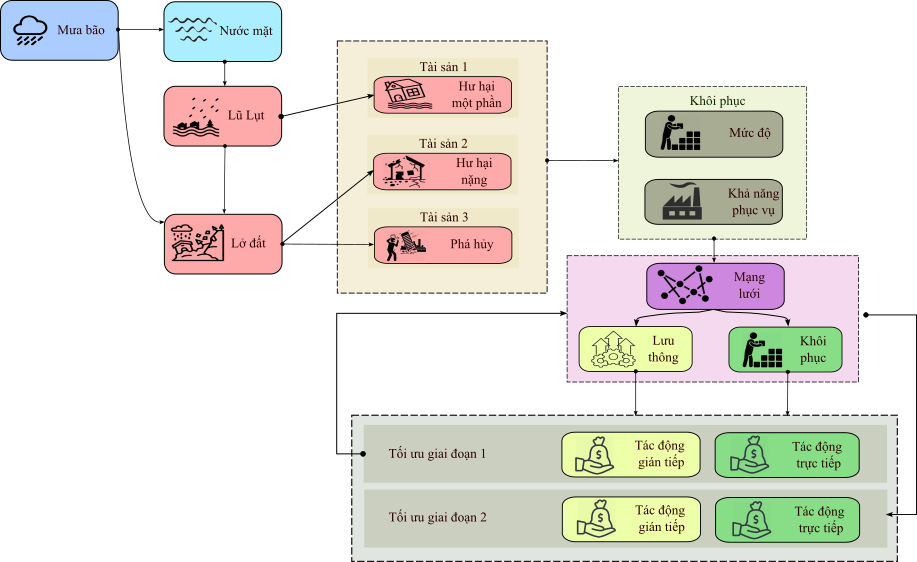
\includegraphics[width=14cm]{restoration}% This is a *.eps file
	\end{center}
	\caption{Phục hồi mạng lưới điện khi có sự cố gây ra bởi thiên tai}\label{fig:restoration}
\end{figure}
\FloatBarrier


\subsection{Phân tích dữ liệu thu thập từ các công tơ thông minh}

Ứng dụng phân tích dữ liệu lớn cho dữ liệu thu thập từ các công tơ thông minh có thể là
\begin{itemize}
\item Các ứng dụng về phân tích dự trên một công tơ thông minh
\item Các ứng dụng về phân tích dự trên nhiều công tơ thông minh
\item Các công tơ thông minh được kết nối với các mô hình mạng lưới
\end{itemize}

Số lượng đồng hồ thông minh được lắp đặt ở Mỹ và Châu Âu đã vượt quá 50\% trên tổng số lượng công tơ điện tính tới thời điểm năm 2020. Điều này hiển nhiên cung cấp cơ hội lớn cho việc phân tích dữ liệu để nâng cao quản lý khách hàng và hoạt động và kế hoạch quản lý lưới điện. Các công tơ thông minh cung cấp các chỉ số về năng lượng, công suất và điện áp ở mức độ phân giải cao, thường là một giờ hoặc 15 phút. Số liệu lấy từ công tơ điện thông minh được sử dụng cho phân tích như dự báo, phân loại tải cho từng đối tượng khách hàng, ước tính tải. Khi kết hợp với các nguồn dữ liệu khác và các hệ thống tiện ích, phân tích dựa trên dữ liệu từ công tơ thông minh có thể được mở rộng và tạo thêm lợi ích cho hoạt động của doanh nghiệp. %Tóm tắt của ứng dụng đồng hồ thông minh được minh họa trong Hình 5.

%Dưới đây, chúng tôi cung cấp một tóm tắt các ứng dụng nổi bật của thông minh phân tích dữ liệu đồng hồ với các tham chiếu tương ứng. Một số ứng dụng sẽ được mở rộng trong các phần tiếp theo dưới các tiêu đề riêng biệt.

%\subsubsection{Dự báo tải}
%Ngành công nghiệp điện đã sử dụng dự báo tải cho hoạt động và kế hoạch lưới và quản lý khách hàng. Dữ liệu đo đạc thông minh đã thu hút sự chú ý của các nhà nghiên cứu trong thập kỷ qua cho cả dự báo tải điểm và xác suất [138,139]. Một xử lý toàn diện hơn về chủ đề này được đề cập trong phần con.

%\subsubsection{Hồ sơ tiêu thụ điện của khách hàng}

%Load profiling đề cập đến phân loại các đọc lịch sử về nhu cầu của khách hàng thành các nhóm dựa trên hành vi của họ. Các kỹ thuật phân cụm như k-means, phân cụm phân cấp và bản đồ tự tổ chức đã được sử dụng cho việc phân loại tải [140-142]. Các mô hình biến thời gian kết hợp với phân cụm đã được sử dụng để phát triển mô hình tải điện phức tạp bằng cách sử dụng dữ liệu Cơ sở hạ tầng Đo lường tiên tiến (AMI) [143]


%\subsubsection{Phân tích DER}
%Một lượng đáng kể các nguồn năng lượng phân tán (DER) đang được kết nối với lưới điện, bao gồm điện mặt trời PV, lưu trữ năng lượng và xe điện. Những nguồn tài nguyên này trong lưới tạo ra những thách thức mới cho các nhà cung cấp tiện ích bao gồm biến động điện áp [144], vi phạm giới hạn nhiệt, dòng ngược và ảnh hưởng đến tuổi thọ dự kiến của cơ sở hạ tầng như máy biến áp và bộ điều chỉnh điện áp. Việc có thông tin chính xác liên quan đến Nguồn năng lượng phân tán (DER) tại mạch phân phối và đằng sau đồng hồ điện (BTM) là rất quan trọng đối với các tiện ích. Các nhà nghiên cứu đã chứng minh khả năng phát hiện điện mặt trời trên mái nhà [145] và xe điện sạc tại đầu tiêu dùng [146] bằng cách sử dụng phân tích không xâm nhập trên dữ liệu đồng hồ thông minh. Các mạng nơ-ron sâu đã được sử dụng để phát hiện kích thước, độ nghiêng và thông số hướng của các cài đặt điện mặt trời dựa trên dữ liệu AMI [147]


%\subsubsection{Các ứng dụng với mạng lưới điện}
%Dữ liệu đồng hồ thông minh có thể được sử dụng kết hợp với dữ liệu nguồn cấp phân phối để có được các mô hình tinh vi cho kế hoạch phân phối hoặc để có được cái nhìn sâu sắc vào các vấn đề mô hình hóa cụ thể. Ví dụ, dữ liệu đồng hồ thông minh đã được sử dụng để phát hiện bất thường [148] như thay đổi đáng kể về nhu cầu hoặc điện áp. Dữ liệu đồng hồ thông minh bị gián đoạn đã được sử dụng cho phân tích và phục hồi gián đoạn tối ưu [149] và thiết kế tái cấu hình nguồn cấp. Phân tích đồng hồ thông minh cũng đã được sử dụng để sửa chữa kết nối biến áp [149], xác định pha [150], xác định độ phức tạp [151] và ước lượng tham số [152]

%\subsubsection{Dự báo tải}
%Trong một cuộc khảo sát phân tích tiện ích được tiến hành vào năm 2017 với 136 tiện ích từ 24 quốc gia, 52\% số người trả lời coi dự báo năng lượng là một ứng dụng ưu tiên cao nhất, tỷ lệ cao nhất trong tất cả các ứng dụng trong cuộc khảo sát [153]. Cải thiện dự báo có thể dẫn đến các quyết định vận hành và kế hoạch tốt hơn và do đó dẫn đến tiết kiệm tiền tệ hoặc nâng cao độ tin cậy của hệ thống. Tùy thuộc vào các yếu tố như kích thước của công ty và mức giảm lỗi, việc giảm lỗi dự báo có thể dẫn đến tiết kiệm hàng triệu đô la mỗi năm [154]. Trong thời đại dữ liệu lớn, sự tăng trưởng của dữ liệu, sự tiến bộ của các công nghệ tính toán và các đột phá trong phân tích tiên tiến tiếp tục kích thích cải tiến các kỹ thuật và phương pháp dự báo năng lượng. Nhiều trong số những phát triển gần đây này đã được công nhận là các giải thưởng trong các Cuộc thi Dự báo Năng lượng Toàn cầu (GEFCom) [42-44].

%Các tiện ích đã thực hành dự báo tải trong hơn một thế kỷ [155]. Theo sự phát triển của lưới điện và ngành công nghiệp điện, dự báo tải dài hạn, hoặc dự báo tải không gian, đặc biệt là đã được coi là một thành phần quan trọng trong kế hoạch hệ thống điện vào cuối thế kỷ 20 đến đầu thế kỷ 21 [156-158], khi dữ liệu tải được thu thập từ các biến áp phân phối và ở độ phân giải thấp, chẳng hạn như hàng tháng hoặc hàng năm. Tuy nhiên, nhu cầu vận hành phức tạp ngày càng đòi hỏi dự báo tải ngắn hạn chính xác [159]. Các kỹ thuật trí tuệ nhân tạo, chẳng hạn như mạng nơ-ron nhân tạo, đã chiếm đa số các tài liệu vào những năm 1990 [160]. Mặc dù nhiều mô hình được phát triển cho Luồng Tải Ngắn Hạn (STLF), nhưng hầu hết đều không có giá trị thực tiễn. Một thành công đáng chú ý phát triển từ giới học thuật vào những năm 1990 là một mô hình mạng nơ-ron, sau đó được thương mại hóa và vẫn được sử dụng trong ngành công nghiệp ngày nay [161]. Một khám phá nghiên cứu học thuật gần đây khác đã được thương mại hóa và triển khai trên toàn cầu trong những năm 2010 là một khung mô hình dựa trên hồi quy [39,162].

%Khi các công nghệ tự động hóa phân phối và lưới điện thông minh cung cấp dữ liệu độ phân giải không gian thời gian cao cho các nhà dự báo tải, nghiên cứu về dự báo tải cũng phát triển mạnh. Ví dụ, các nhà cung cấp điện bán lẻ bắt đầu sử dụng dữ liệu hàng giờ cho dự báo tải dài hạn. Một số nhà khai thác thị trường và tiện ích cũng dựa vào dữ liệu hàng giờ hoặc hàng phút để dự báo tải ở mức điện áp cao [38,39,164]. Những dữ liệu tải có độ phân giải cao này cho phép các nhà dự báo xây dựng mô hình với hàng trăm thông số có thể bắt được nhiều đặc trưng quan trọng trong tải [37]. Chúng cũng cho phép các nhà dự báo tải cải thiện dự báo tổng thể bằng cách tận dụng thông tin tải cấp đồng hồ. [138].

%Trong khi khai thác việc sử dụng dữ liệu tải có độ phân giải cao, các nhà nghiên cứu và chuyên gia cũng đầu tư một số nỗ lực vào các cách sáng tạo để khai thác dữ liệu thời tiết. Truyền thống, chỉ có một số lượng nhỏ các trạm thời tiết được sử dụng để dự báo tải trên một khu vực cụ thể. Tại GEFCom2012, chuỗi nhiệt độ từ 11 trạm thời tiết đã được công bố cho cộng đồng nghiên cứu [42]. Một phương pháp lựa chọn trạm thời tiết sau đó được đề xuất và cho thấy giá trị trong việc cải thiện dự báo tải tiên tiến nhất. Phương pháp này sau đó đã được sử dụng bởi một đội chiến thắng tại GEFCom2014 [165]. Gần đây, nó đã được cải thiện thêm bởi các nhà nghiên cứu khác [166,167]. Vì dữ liệu thời tiết có thể được sử dụng cho nhiều mô hình dự báo tải, các phương pháp lựa chọn trạm thời tiết này có lợi cho cả dự báo tải dài hạn và ngắn hạn.

%Trong khi xu hướng nghiên cứu dự báo tải chính là tận dụng dữ liệu lớn, một xu hướng khác là nhúng thông tin toàn diện về tương lai vào dự báo tải. Dự báo tải xác suất, cung cấp dự báo theo phân vị, khoảng xác suất hoặc hàm mật độ, là chủ đề nóng trong thập kỷ qua [168]. Những dự báo tải xác suất này có thể được tạo ra thông qua mô phỏng phần dư [169,170], tạo ra các kịch bản đầu vào [171] hoặc kết hợp dự báo điểm [172]. Hồi quy phân vị cũng đã được áp dụng để tạo ra dự báo tải xác suất [139,172,173]. Một số khía cạnh phương pháp của dự báo cũng đã được nghiên cứu đặc biệt cho dự báo tải xác suất, chẳng hạn như lựa chọn đặc trưng [174,175] và kết hợp dự báo [176].

%Ngoài việc cải thiện dự báo tải ở mức điện áp cao, các nhà nghiên cứu và chuyên gia cũng đã dành nhiều nỗ lực cho dự báo tải ở mức điện áp trung bình và thấp. Một số dự báo tại mức điểm cung cấp [42, 44], trong khi những người khác là ở các đồng hồ đo riêng lẻ [40, 139, 177]. Chủ đề phổ biến khác là dự báo tải cho tòa nhà, từ các tòa nhà học thuật [178, 179] đến các tòa nhà dân cư [180, 181]. Trong khi thời tiết vẫn đóng vai trò chính trong nhiều mô hình dự báo tải ở mức tòa nhà, tác động của thời tiết đối với tải công nghiệp là khá nhỏ. Dự báo tải cho nhà máy và các cơ sở công nghiệp là một chủ đề mới nổi trong loại này [182-184], và bao gồm dự báo tải công suất phản kháng.

\subsection{Dự báo và phân tích năng lượng tái tạo}
%Việc triển khai năng lượng tái tạo đã tiếp tục được duy trì với tốc độ ổn định trong thập kỷ qua. Do tính không đồng nhất của việc tạo điện từ các nguồn năng lượng tái tạo, cũng như do sự khó lường hạn chế, sự chú trọng đã được đặt vào việc phát triển các phương pháp tích hợp những nguồn tái tạo đó. Ngoài các khía cạnh liên quan đến mã lưới điện và một số phương pháp quản lý năng lượng phân tích mới được đề cập trong các phần khác, một phần lớn nỗ lực đã tập trung vào cách tận dụng tối đa các dữ liệu có sẵn để cải thiện kiến thức về việc tạo điện từ nguồn năng lượng tái tạo, thường là với mục đích dự báo. Một trong những bài báo đầu tiên đề xuất mô hình động để dự đoán tốc độ gió và sản lượng điện tương ứng là [185]. Mặc dù tập trung vào các mô hình đơn giản và một bố cục ảo, bản thảo đó đã đặt nền tảng cho một số phát triển tiếp theo. Rõ ràng, vào thời điểm đó, các khía cạnh dữ liệu lớn chưa được thảo luận, và số chiều của các mô hình liên quan cũng nhỏ.

Ngày nay tại các trang trại điện gió, đặc biệt là các trang trại điện gió ngoài khơi, việc thu thập dữ liệu ở mức độ động cơ gió được thực hiện với độ phân giải một giây. Tương tự, đối với các nhà máy năng lượng mặt trời, dữ liệu có thể được thu thập ở mức độ biến tần và với độ phân giải cùng cấp độ giây \citep{Gilbert2020}. Những dữ liệu ở mức độ rất tinh vi này được sử dụng để cải thiện phân tích và dự báo. Ngoài ra, vì khả năng sinh năng lượng từ các nguồn tái tạo bắt đầu trở nên đa dạng và phân tán địa lý một cách dày đặc, ta cũng có thể sử dụng tất cả dữ liệu được thu thập tại các trang trại để cải thiện dự báo.

Ngoài ra, còn có rất nhiều nguồn dữ liệu khác có liên quan, chủ yếu là liên quan đến quan sát và dự báo khí tượng, mô tả các quy trình phức tạp và mang lại khối lượng dữ liệu rất lớn. %Về phía cạnh quan sát khí tượng:

\begin{itemize}
\item Sky imagers có tiềm năng lớn cho mô hình hóa và dự báo năng lượng mặt trời với độ phân giải cao vì chúng theo dõi các đám mây di chuyển và tác động của chúng đến các tấm pin mặt trời \citep{Chow2011}. Chúng có thể cung cấp hình ảnh của bầu trời trên các nhà máy điện mặt trời mỗi 30 giây;

\item Radar thời tiết cũng đã chứng minh tầm ảnh hưởng trong đánh giá và mô hình hóa các chế độ làm việc của các trang trại điện gió. Tùy thuộc vào công nghệ, hình ảnh radar có thể có sẵn giữa mỗi phút và mỗi 10 phút, với bán kính hình ảnh từ 60 đến 250 km;

\item Dữ liệu từ LIDAR ngày càng được coi là rất liên quan đến các đo lường gió ở phía trước của các tuabin gió và chúng được tích hợp vào các phương pháp dự báo, hoặc nói chung là các quan sát tiềm năng mới về gió được sử dụng trong dự báo thời tiết và năng lượng tái tạo. LIDAR cung cấp các đo lường gió cho hình nón mà chúng quét (theo chiều dọc hoặc chiều ngang, tùy thuộc vào cách chúng được thiết lập) mỗi vài giây.
\end{itemize}

Ngoài ra, có thể đề cập đến hình ảnh vệ tinh, có tiềm năng quan trọng cho năng lượng gió, mặt trời và sóng. Tuy nhiên, tần suất cập nhật thấp hơn khiến chúng ít quan trọng hơn ở thời điểm hiện tại. Thông tin từ các loại thiết bị này được gọi là thông tin được cảm biến từ xa.

%Một thách thức đầu tiên và phức tạp khi xử lý thông tin cảm biến từ xa là giảm chiều. Điều này có thể được thực hiện: (i) dựa trên các kỹ thuật xử lý tín hiệu và thống kê, ví dụ như Phân tích thành phần độc lập-ICA, cho các trường chuyển động trong hình ảnh radar thời tiết; (ii) bằng cách trích xuất các đặc trưng vật lý như mây trong hình ảnh bầu trời [188] hoặc hệ thống mưa và đặc điểm của chúng trong hình ảnh radar [192]; hoặc cuối cùng (iii) thông qua các mô hình chức năng như các hồ sơ gió cho các đo đạc dọc theo chiều dọc của LiDAR.

%Ngoài các quan sát khí tượng, dữ liệu đầu vào chiều cao mới có thể có dạng dự báo thời tiết. Trước hết, thông tin liên quan trong dự báo thời tiết không chỉ có thể dành cho điểm gần nhất với một điểm quan tâm mà còn có thể được cung cấp trên toàn khu vực của điểm đó [59]. Thứ hai, để diễn đạt dự báo theo cách xác suất, các dự báo thời tiết tập hợp bao gồm một tập hợp các quỹ đạo thay thế và có khả năng như nhau (thông thường, giữa 10 và 100) cho các biến thời tiết liên quan. Chúng có thể được hiểu là các thực hiện mẫu từ các dự báo xác suất đa biến để cung cấp cho các phương pháp dự báo năng lượng tái tạo. Chúng có sẵn trên các khu vực lớn. ví dụ, toàn bộ châu Âu, cung cấp thông tin về phụ thuộc không gian-thời gian đa biến trong việc tạo điện năng tái tạo [193,194]. Cuối cùng, dự báo thời tiết độ phân giải rất cao (độ phân giải không gian trong khoảng vài mươi đến vài trăm mét và độ phân giải thời gian trong khoảng vài giây đến vài phút) đang mang lại cơ hội mới cho dự báo năng lượng tái tạo, như trong ví dụ gần đây trong [186] và các ứng dụng tại các trang trại gió ngoài khơi.

Hiện nay, sự sẵn có của số lượng lớn dữ liệu này yêu cầu những thay đổi cơ bản trong phân tích và dự báo năng lượng tái tạo, không chỉ về phương pháp mà còn về các mô hình kinh doanh. Chúng ta mong đợi sẽ có nhiều công trình đổi mới xuất hiện trong tương lai, đề xuất các phương pháp dựa trên phương trình vi phân ngẫu nhiên, học sâu, học phân tán và liên kết, cũng như dữ liệu về thị trường.


\subsection{Hiệu quả và tối ưu hóa năng lượng}
Các công nghệ về lưới điện thông minh cung cấp tiềm năng lớn để tăng cường hiệu quả sử dụng năng lượng trong các lĩnh vực khác nhau. Tuy nhiên, hiện tại, các hoạt động tăng cường hiệu quả năng lượng chủ yếu bị hạn chế trong việc thực thi tiêu chuẩn ISO 50001 như: (i) lắp đặt thiết bị bổ sung (đồng hồ đo, cảm biến, v.v.) để đo lường tiêu thụ năng lượng; (ii) lắp đặt phần cứng mới và thay thế thiết bị; và (iii) trực quan hóa dữ liệu, tìm các mô hình bất thường; và xác định các quy trình tiêu thụ năng lượng cao. Thực tiễn tiêu chuẩn này cung cấp việc giám sát và nhận thức về tiêu thụ năng lượng cho các quyết định của con người, nhưng nó không cho phép phân tích theo chỉ đạo và kiểm soát quy trình tự động.

%Các tác phẩm khác nhau trong văn học khai thác các kỹ thuật tối ưu hóa năng lượng dựa trên mô hình, chẳng hạn như lập trình số nguyên cho việc giảm tải đỉnh trong các nhà máy thép [195] và lập trình tuyến tính số hỗn hợp cho các thiết bị gia dụng nhiệt [196]. Các phương pháp dựa trên mô hình có nhược điểm là yêu cầu một mô hình (toán học) về quá trình vật lý và các ràng buộc, có thể phức tạp trong một số trường hợp. Chúng không cho phép cải tiến liên tục các chính sách kiểm soát.

Sự xuất hiện của công nghệ internet-of-things cung cấp điều kiện kỹ thuật cho mô hình hóa động lực dữ liệu trong tối ưu hóa năng lượng. Một số ví dụ là việc sử dụng học tăng cường dạng batch (fitted Q-iteration) để điều khiển một nhóm máy sưởi nước điện gia đình cho dịch vụ đáp ứng nhu cầu \citep{Ruelens2014}; fitted Q-iteration kết hợp với auto-encoders để tối ưu hóa năng lượng trong máy sưởi nước điện \citep{Ruelens2018}; học tăng cường sâu cho tối ưu hóa năng lượng dự đoán các trạm bơm nước thải \citep{Filipe2019}; và mô hình cây cho tiêu thụ năng lượng của tòa nhà để lên lịch hệ thống sưởi ấm tối ưu \citep{Kouzelis2015}. Phương pháp này không yêu cầu việc mô hình hoá đầy đủ các phương trình quá trình vì sự hiểu biết của nó được thực hiện theo thời gian thực thông qua dữ liệu. Tuy nhiên, sẵn có dữ liệu và thời gian (ví dụ: số lần tương tác với hệ thống vật lý) cần thiết để "huấn luyện" các phương pháp tối ưu dữ liệu vẫn là thách thức thực tế cho sự áp dụng trong ngành công nghiệp.

%Ngoài tối ưu hóa năng lượng dữ liệu, các dịch vụ năng lượng dựa trên dữ liệu khác có thể được cung cấp bởi các công ty dịch vụ năng lượng (ESCO), nhà tập đoàn và nhà bán lẻ nhằm tối đa hóa nhận thức của người sử dụng cuối đối với các hành động tăng hiệu quả sử dụng năng lượng và rút ra giá trị kinh doanh từ dữ liệu.

%Một đóng góp quan trọng để tăng sự nhận thức của người sử dụng cuối là giám sát tải không xâm phạm từ dữ liệu của các công tơ thông minh, có thể được áp dụng để phát hiện và ước tính các cài đặt điện PV dân dụng [145], tiêu thụ bơm nhiệt [201] và các hồ sơ tải cá nhân từ các đường cong tải nguồn [202]. Phân đoạn khách hàng với các hồ sơ tải có thể được áp dụng bởi các nhà tập đoàn và nhà bán lẻ để xác định khách hàng mục tiêu, thiết kế một loại giá động hoặc thời gian thực tùy chỉnh [203], mô hình hóa hành vi động của các tải/công tắc có thể kiểm soát được [204], hoặc thông báo cho người tiêu dùng nếu họ đang đối mặt với một sự thay đổi không bình thường của hồ sơ tải. Các kỹ thuật tiêu chuẩn là phân cụm chuỗi thời gian lô, nhưng phân cụm trực tuyến là một yêu cầu cơ bản do tính động của hành vi tiêu thụ [205].

%Dữ liệu từ đồng hồ đo thông minh kết hợp với các biến môi trường bên ngoài (ví dụ: nhiệt độ ngoài trời) có thể hỗ trợ cho các nhà bán lẻ và nhà tổng hợp ước tính khả năng phản ứng yêu cầu của khách hàng. Trong [206], một vấn đề bao lưu ngẫu nhiên được đặt ra để lựa chọn khách hàng trong các chương trình phản ứng yêu cầu sử dụng dữ liệu tiêu thụ, cũng như để ước tính xác suất đạt được mục tiêu giảm tải. Các phương pháp suy luận nhân quả giữa các chương trình tính tiền Nguồn Phân tán (DR) và tiêu thụ được sử dụng trong [207] để ước tính độ đàn hồi của người tiêu dùng và xác định liệu các chương trình tính tiền động có ảnh hưởng đến sơ đồ tiêu thụ thông thường của người tiêu dùng hay không; mục tiêu tương tự cũng được đạt được với phương pháp dựa trên tương quan [208]. Hơn nữa, học trực tuyến có thể được sử dụng để điều chỉnh tín hiệu giá động để đạt được hành vi sử dụng mong muốn, ví dụ, bằng cách đặt ra một vấn đề tối ưu lồi trực tuyến [209] hoặc thông qua một mô hình tiện ích tham số hóa [210].


%Dữ liệu được thu thập từ đánh giá và chứng nhận hiệu quả năng lượng rất có giá trị cho các bên liên quan và dịch vụ khác nhau [211]. Ví dụ, Cơ quan Năng lượng (DOE) cơ sở dữ liệu hiệu suất tòa nhà có thể được sử dụng cho các mục đích khác nhau [212]: so sánh hiệu suất tiết kiệm năng lượng của các loại tòa nhà khác nhau và địa điểm địa lý; ước tính tiềm năng tiết kiệm năng lượng liên quan đến các hành động cải tiến cụ thể; và đánh giá tác động của các công nghệ tiết kiệm năng lượng ở mức độ danh mục. Trên thực tế, các kỹ thuật dựa trên dữ liệu có thể được sử dụng để đánh giá trước các biện pháp cải tiến năng lượng về mặt tiết kiệm năng lượng và "giảm rủi ro" đầu tư vào công nghệ tiết kiệm năng lượng. Ví dụ, hồi quy đa tuyến có thể sản xuất một ước tính xác suất về lợi nhuận liên quan đến các biện pháp cải tiến khác nhau, xem xét các đặc điểm và hệ thống của tòa nhà [213].


%\subsection{Phân tích dữ liệu synchrophasor và sự kiện}
%Để đánh giá tầm quan trọng của dữ liệu Đơn vị Đo Pha (PMU), ta phải trở về các báo cáo về nguyên nhân của sự cố mất điện lớn tại đông bắc Hoa Kỳ vào ngày 13 tháng 8 năm 2003 [214]. Ban Nghiên cứu Sự cố Hệ thống Điện quốc tế Hoa Kỳ-Canada đã kết luận rằng một trong những lý do chính dẫn đến sự cố mất điện là thiếu nhận thức về tình hình thực tế. Điều này, lần lượt, được cho là do tầm nhìn hạn chế của nhà điều hành về các sự kiện và động lực liên quan đến hệ thống điện được cung cấp bởi Hệ thống Quản lý Năng lượng (EMS) thông qua các thiết bị đo trường như hệ thống Giám sát và Thu thập Dữ liệu (SCADA) và các thiết bị ghi lại tại trạm biến áp như máy ghi sự cố kỹ thuật số, máy bộ định hướng kỹ thuật số và máy ghi sự kiện trình tự. Thiếu sót chính là tốc độ báo cáo đo đạc (Đơn vị Trung tâm Tầm xa SCADA), thiếu dấu thời gian khác biệt (cơ sở dữ liệu SCADA) và không thể cập nhật mô hình hệ thống điện kịp thời để phản ánh các sự kiện chuyển mạch liên tiếp (bộ ước lượng trạng thái). Ngoài ra, các thiết bị ghi sự cố không được đồng bộ thời gian và đánh dấu thời gian đầy đủ. Để khắc phục những thiếu sót đó, các PMU và hạ tầng đo đạc phụ thuộc vào synchrophasor được xác định là cơ sở đo lường phù hợp. Với sự tăng cường nguồn kinh phí từ Đạo luật Phục hồi và Tái đầu tư Hoa Kỳ năm 2009, nhiều PMU đã được lắp đặt trên khắp Hoa Kỳ và hiện đang có hơn 2.500 đơn vị. Một số lượng PMU ngay cả lớn hơn đã được lắp đặt tại Trung Quốc và đang tiến hành kế hoạch lắp đặt một số lượng lớn tại Ấn Độ.

%Một trong những điểm mạnh chính của PMU là cung cấp các phép đo đồng bộ thời gian của phasor điện áp và dòng điện thời gian thực với tốc độ báo cáo cao hơn đáng kể so với các Đơn vị Điều khiển Từ xa SCADA (RTU). Có thể hiểu được cách thức thực hiện này thông qua Hình 6, trong đó hiển thị kiến trúc tổng quát của PMU. Các đặc tính chính của PMU là xung một lần mỗi giây (1PPS) và mã thời gian được cung cấp bởi bộ đếm thời gian toàn cầu GPS. Tín hiệu đồng hồ chính xác với tốc độ 1PPS cung cấp cho mạch lấy mẫu và giữ (S/H) ở tất cả các PMU, cho phép đồng bộ lấy mẫu của các dạng sóng đầu vào trên không chỉ các đầu vào của một PMU mà là đầu vào của tất cả các PMU được lắp đặt trong một hệ thống điện cụ thể. Mã thời gian đại diện cho thời gian tuyệt đối cung cấp khả năng đánh dấu thời gian tham chiếu cho tất cả các giá trị phasor được tính toán. Các giá trị phasor tính toán như vậy được báo cáo với tốc độ mỗi giây là 30, 60, 120 hoặc thậm chí cao hơn, cung cấp hai lợi thế chính: a) cung cấp dữ liệu chất lượng cao với tốc độ dữ liệu cao, và b) đảm bảo tính toán độ chênh lệch pha chính xác cao giữa bất kỳ vị trí nào trong hệ thống và phasor tham chiếu.

%Điều này cung cấp một cơ hội độc đáo cho phân tích sau sự kiện, đặc biệt là trong trường hợp các sự kiện phức tạp (ví dụ: lỗi lan truyền do sự cố thiết bị dẫn đến mất điện). Ngoài ra, việc bắt và phân tích các dao động trong hệ thống điện quan trọng vì nó báo hiệu về khả năng sụp đổ của hệ thống [216]. PMU đóng vai trò quan trọng trong việc ghi nhận các sự cố [217] với sự phát triển gần đây của các công nghệ xác định và phân loại sự cố [217-220]. Trong những năm gần đây, khả năng của hệ thống điện đã được mở rộng để bao gồm các nguồn năng lượng tái tạo, nhu cầu năng lượng tăng, tích hợp xe điện, vv. Tất cả các công nghệ này đều đặt ra những thách thức mới cho hoạt động hệ thống. Dữ liệu PMU cung cấp một nguồn thông tin có giá trị có thể giúp đáp ứng các thách thức và tăng cường sự phù hợp của lưới kết hợp.

%Do đó, dữ liệu được thu thập từ PMU đóng một vai trò quan trọng trong các ứng dụng như giám sát, điều khiển, bảo vệ, ước lượng trạng thái, đánh giá sự ổn định và phát hiện sự cố [221]. Tuy nhiên, phân tích sau sự kiện vẫn được thực hiện bằng tay trong nhiều trường hợp với khả năng dự đoán hạn chế hoặc không có. Các kỹ thuật được đề xuất trong các giải pháp phần mềm được nhắc đến nhằm mục đích phân tích tự động có khả năng không chỉ phân loại các sự kiện quá khứ mà còn dự đoán những trường hợp sự cố trong tương lai sử dụng các bản ghi dữ liệu trực tiếp.

%Phần lớn các phương pháp dự đoán cho phân tích dữ liệu PMU trong văn bản tập trung vào việc cho phép nhận thức tình huống có ý nghĩa hơn so với những gì được bao phủ bởi EMS SCADA, từ đó đảm bảo sự ổn định động của hệ thống [222-229]. Các phương pháp dự đoán có thể mở rộng khả năng phân biệt các loại sự kiện của các nhà điều hành, từ hoạt động bình thường đến hoạt động trong điều kiện cực đoan bằng cách bắt giữ các đặc trưng dạng sóng PMU và tự động xác định các sự kiện trong quá trình phân loại. Điều này cho phép ứng dụng của dữ liệu lớn, trí tuệ nhân tạo và học máy giúp đoán trước nhiều loại cảnh báo và sự cố khẩn cấp trong hệ thống điện, ngoài việc theo dõi hoạt động bình thường và cực đại ổn định động lực. Kiến thức ban đầu có thể được sử dụng như hướng dẫn cho nghiên cứu tương lai trong lĩnh vực này và có thể mở cánh cửa cho khám phá sâu hơn của các thuật toán dự đoán dựa trên PMU cho các ứng dụng khác, chẳng hạn như quản lý và giám sát tài sản hoặc dự đoán và quản lý sự cố.

%Một thách thức mà tất cả các đơn vị liên quan đến phát triển các ứng dụng trực tuyến và ngoại tuyến đều đang đối mặt là sự gia tăng của một lượng dữ liệu rất lớn đến từ PMUs. Để cải thiện tính tin cậy, bảo mật và hiệu quả của hệ thống, cần phát triển các công cụ tự động có khả năng phân tích các sự kiện quá khứ và thông báo quyết định trong thời gian thực. Điều này có nghĩa là các phương pháp đề xuất cần phân biệt giữa các kỹ thuật phù hợp để truy cập và xử lý một lượng lớn dữ liệu lịch sử, trong đó thời gian xử lý không quan trọng bằng các kỹ thuật nhằm vào xử lý dữ liệu luồng trong thời gian thực, trong đó tính hiệu quả tính toán là rất quan trọng.

%Khi tài nguyên tính toán tiến bộ, việc học và trích xuất các mẫu hữu ích từ dữ liệu lớn tạo ra cơ hội mới. Học sâu [88,92,93] cho phép tìm thấy các mẫu trừu tượng hơn từ dữ liệu phức tạp lớn, thậm chí là không đồng nhất [230]. Một mô hình sâu học một cách đa tầng. Mỗi khi dữ liệu mới hoặc tập các đặc trưng được truyền qua một tầng, một cấp độ trừu tượng dữ liệu mới được giới thiệu. Do đó, thông qua nhiều tầng liên tiếp, các mô hình sâu học được học các biểu diễn giàu, cấp cao của dữ liệu thô cấp thấp như hình ảnh, âm thanh và văn bản. Nói cách khác, các mô hình sâu cung cấp một khung việc toàn diện cho việc trích xuất đặc trưng tự động, phức tạp ở một cấp độ trừu tượng cao. Các mô hình sâu không trích xuất các biểu diễn được xác định trước - ngược lại, chúng có xu hướng tìm ra các mẫu không thay đổi bằng cách loại bỏ sự biến động trong dữ liệu [231]. Giả thuyết cuối cùng trong vấn đề này cho rằng càng nhiều dữ liệu, càng trích xuất được nhiều kiến thức [232], và do đó khả năng tổng quát hóa càng lớn hơn có thể đạt được. Các biểu diễn được học là rất gọn nhẹ, giúp giảm thiểu tính toán và từ đó làm cho việc học tiếp theo rất hiệu quả.

%Kiến trúc tổng quan của quá trình phân tích dữ liệu PMU tự động được trình bày trong Hình 6.


%\subsection{Các ứng dụng cho lưới điện}
%Sự đầu tư vào các công nghệ Lưới điện Thông minh (ví dụ như đồng hồ thông minh, PMU và các thiết bị điện tử thông minh [IED]) cho lưới điện phân phối và truyền tải đang cải thiện khả năng giám sát và điều khiển của chúng \citep{Simoes2012}. Đồng thời, các khung pháp lý và thị trường mới đang được thử nghiệm (ở cấp độ thử nghiệm) và triển khai ở các quốc gia khác nhau để hỗ trợ tích hợp các nguồn điện phân tán linh hoạt.

%\subsubsection{Tính quan sát}
%Mặc dù có tất cả những tiến bộ công nghệ, khả năng quan sát lưới điện áp thấp (LV) vẫn là một trở ngại chính để khai thác tối đa tiềm năng từ những công nghệ này và tích hợp các nguồn điện phân tán linh hoạt vào thị trường điện và quản lý hệ thống điện. Điều này có thể được chia thành hai thách thức chính: (i) đặc trưng của địa hình (topo) và các thông số lưới điện; và (ii) giám sát thời gian thực.

%Thông tin từ các đồng hồ thông minh được lắp đặt tại khách hàng áp thấp và trạm phân phối cấp hai có thể được sử dụng để xây dựng topo lưới sử dụng nhiều phương pháp khác nhau, chẳng hạn như: mô hình đồ thị xác suất và hồi quy tuyến tính LASSO [234, 235]; và luồng điện kết hợp với thông tin chung [151]. Trong một số trường hợp, thông tin về tôpô lưới có sẵn, nhưng các thông số điện có sai số lớn hoặc không biết (tức là sử dụng các thông số từ các danh mục dây cáp), và do đó, cần thực hiện một ước lượng chắc chắn (và dựa trên dữ liệu) của các thông số lưới [236, 237]. Vấn đề này cũng yêu cầu phát triển các phương pháp để lập kế hoạch vị trí cảm biến và giảm thiểu chi phí giám sát [238]. Một nguồn không chắc chắn khác là giai đoạn kết nối của mỗi khách hàng. Gom nhóm các phép đo độ lớn điện áp 15 phút từ các đồng hồ thông minh có thể xác định các nhóm khách hàng được kết nối với cùng một giai đoạn và giảm chi phí nhân công cho việc xác định giai đoạn trên thực địa [239]. Dữ liệu của đồng hồ thông minh cũng có thể được sử dụng để ước tính công suất định mức của các tấm pin năng lượng mặt trời cài đặt sau đồng hồ [240] và phát hiện xe điện đang sạc [241].

%Về mặt giám sát thời gian thực, thông tin về hồ sơ điện áp là rất quan trọng để tạo ra các cảnh báo cho các nhân viên vận hành tại các trung tâm phân phối điện áp thấp. Tuy nhiên, ngay cả với các giao thức truyền thông như Power Line Communication (PLC) PRIME hoặc General Packet Radio Service (GRPS), việc thu thập thông tin 15 phút một lần từ hàng trăm khách hàng là không khả thi hoặc chi phí truyền thông rất cao. Các chức năng ước tính trạng thái dựa trên dữ liệu giúp ước tính độ lớn điện áp tại mỗi nút điện áp thấp trong thời gian thực chỉ bằng cách sử dụng thông tin từ một tập hợp con các đồng hồ thông minh (tức là 10-20\%) có khả năng truyền thông thời gian thực [242]. Dự báo tải và sản xuất có thể được sử dụng như đầu vào trong thuật toán ước tính trạng thái tiêu chuẩn và tạo ra một ước tính xác suất của điện áp nút [243].


%Các mức điện áp khác cũng được hưởng lợi từ các chức năng ước tính trạng thái dựa trên dữ liệu để giám sát thời gian thực. Một số ví dụ bao gồm: một chức năng ước tính trạng thái dựa trên dữ liệu mạnh mẽ được đề xuất trong [244] để khai thác dữ liệu lịch sử được thu thập bởi các đồng hồ đo phân phối và PMU, bằng cách tìm các đặc trưng tương đồng trong một khung làm việc học có giám sát với hồi quy kernel ridge; một bộ ước tính trạng thái động có khả năng dự báo được mô tả trong [245]; kết hợp dữ liệu SCADA từ các trạm phân phối chính (thông thường có sẵn trong cơ sở dữ liệu trung tâm với độ trễ vài giây/phút) và trạm phân phối phụ (thông thường có sẵn trong cơ sở dữ liệu trung tâm với độ trễ một vài giờ) có thể suy ra điều kiện vận hành gần thời gian thực của lưới điện áp trung bình (MV) [246,247]; và một khối ghép của các bộ tự mã hóa cạnh tranh địa phương ước tính trạng thái của các công tắc lưới dựa trên một tập hợp các đo lường điện cục bộ [248]. Hơn nữa, các chức năng truyền thống, chẳng hạn như phát hiện cục bộ, cũng có thể được hưởng lợi từ các chức năng phân tích dữ liệu tích hợp thông tin văn bản, thời gian và không gian từ các phương tiện truyền thông xã hội [21] và dữ liệu PMU [218].



%\subsubsection{Hộ trợ ra quyết định và điều khiển}
%Các chức năng dựa trên dữ liệu cũng đang được tích hợp vào các hệ thống quản lý năng lượng truyền thống (EMS) và quản lý phân phối (DMS) để bổ sung hoặc thay thế các chức năng phân tích lưới điện truyền thống như lưu lượng điện, cấu hình mạng, lưu lượng điện tối ưu, vv. Trong một số trường hợp, một mô hình học máy được sử dụng như là một proxy cho các chức năng truyền thống, ví dụ như ước tính lưu lượng điện của ma trận Jacobian với dữ liệu PMU [249] và tính toán cam kết đơn vị [250]. Một điểm bất lợi tiềm tàng của phương pháp này là cần thu thập hoặc mô phỏng một bộ dữ liệu lớn để vừa với các mô hình. Tuy nhiên, sau khi được vừa, nó có thể được tích hợp vào các ứng dụng khác nhau và cung cấp các ước tính nhanh chóng.


%Trong những trường hợp khác, học máy được sử dụng để học từ dữ liệu lịch sử về các hành động điều khiển của các nhà điều hành và hỗ trợ ra quyết định [251] hoặc để khám phá các giải pháp mới (và tốt hơn) bằng cách sử dụng các hệ thống chuyên gia [252]. Một lợi thế quan trọng của hai phương pháp này, được phát triển cho Chủ sở hữu Hệ thống Truyền tải (TSOs), là tính giải thích cao đối với những người ra quyết định và khả năng khai thác kiến thức chuyên gia (tức là quyết định quá khứ và các heuristics điều khiển). Tuy nhiên, cả hai đều thuộc mô hình học bằng mô phỏng, tức là học có giám sát được áp dụng cho các quyết định từ chuyên gia, và không khám phá (hoặc tìm kiếm) các giải pháp mới. Một lựa chọn khác là học tăng cường, cung cấp một sự đánh đổi giữa khai thác và khám phá và trong một số trường hợp, như trường hợp được mô tả trong [253], có thể kết hợp với học bằng mô phỏng.

%Một số trường hợp sử dụng cho phương pháp điều khiển dữ liệu này là: xếp hạng nhanh các trường hợp dự phòng cấp cao hơn (theo nguy cơ của chúng) để ưu tiên mô phỏng hệ thống điện năng [254]; và phân tích nhân quả trên dữ liệu đo lường để thực hiện các chiến lược tấn công node tối ưu [255].

%Cuối cùng, việc tích hợp các hệ thống năng lượng tái tạo và sự áp dụng rộng rãi của IEC 61850 đang tăng thêm khối lượng dữ liệu cảnh báo và số lượng cảnh báo đòi hỏi sự chú ý và hành động điều khiển trong phòng điều khiển [256]. Các phương pháp truyền thống dựa trên hệ thống chuyên gia dựa trên quy tắc [257], nhưng thiếu khả năng cung cấp những thông tin bổ ích về các thông tin chứa trong chuỗi cảnh báo và giảm tải trí nhớ của nhân viên điều khiển. Trong [258], một kỹ thuật phân loại thô không giám sát được đề xuất để giảm khối lượng dữ liệu và thông báo nhận được tại các trạm biến áp trong các tình huống khẩn cấp và cải thiện quyết định, nhưng không cung cấp đề xuất về hành động điều khiển. Bước quyết định cuối cùng này (tức là xác định một chuỗi các thao tác thủ công bởi người điều khiển) thiếu trong hầu hết các phương pháp xử lý dữ liệu từ các hệ thống bảo vệ và là một yếu tố cốt lõi để tạo ra tác động thực sự từ các chức năng phân tích dữ liệu, chẳng hạn như giảm thời gian để đưa ra quyết định đầu tiên và chỉ số thời gian gián đoạn trung bình của hệ thống (SAIDI).

\section{Cơ hội và thách thức trong tương lai}

%Cuộc khảo sát cho thấy có nhiều ứng dụng đang ở các giai đoạn thực hiện thực tế khác nhau. 

%Trong khi số lượng tài liệu tham khảo về chủ đề tổng quan về dữ liệu lớn đã rất lớn, dự kiến công việc sẽ tiến triển với tốc độ chưa từng có, và số lượng tài liệu tham khảo sẽ tiếp tục tăng trong tương lai gần.

%Tuy nhiên, trong một số cuộc khảo sát đã công bố, không rõ ứng dụng cuối cùng của một số kỹ thuật được khảo sát là gì, và lợi ích và động lực kinh doanh liên quan là gì. Chúng tôi nhận thấy lợi ích của nghiên cứu tương lai là tập trung vào các ứng dụng cuối cùng trong khi đồng thời giải quyết các vấn đề cơ bản để thúc đẩy những cơ hội sau đây cuối cùng:
Các thách thức và cơ hội liên quan đến công tác phân tích dữ liệu lớn trong tương lai có thể được tóm tắt theo liệt kê dưới đây:
\begin{itemize}
\item Dự đoán các sự kiện trước thời gian và cho phép triển khai các chiến lược giảm thiểu rủi ro và tính toán rủi ro.

\item Tối ưu hóa sử dụng dữ liệu đã thu thập cho lợi ích của doanh nghiệp và người sử dụng. Kết hợp mô hình vật lý và dữ liệu để cải thiện việc phân tích nguyên nhân gốc rễ của các vấn đề. Ngăn chặn các sự cố và hạn chế trong vận hành hệ thống điện hiện tại liên quan đến tác động và hậu quả kinh tế lớn.

\item Thông báo cho người dùng về những hạn chế cung cấp điện sắp tới và sử dụng các nguồn lực phân tán hiệu quả hơn để giảm thiểu sự cố và những tình huống khẩn cấp khác.

\item Thúc đẩy sự đổi mới bằng cách sử dụng kinh nghiệm đa ngành từ các lĩnh vực khác nhau nhưng có mối liên hệ mạnh về thuộc tính dữ liệu và yêu cầu phân tích.

\item Sử dụng dữ liệu từ nhiều nguồn phổ biến khác nhau như máy tính bảng, điện thoại thông minh và các thiết bị điện tử cá nhân khác, khiến doanh nghiệp và các bên liên quan của doanh nghiệp phân tích dữ liệu trở thành các chủ thể cùng tham gia.

\item Thay thế một số nhiệm vụ được thực hiện bởi các nhà điều hành và chuyên gia ngày nay bằng các thuật toán và quy trình tự động hóa.

\item Xây dựng được các mô phỏng không gian và thời gian liên quan đến sự xuống cấp tài sản thiết bị và mạng lưới, đồng thời tích hợp định lượng nguy cơ rủi do, tổn thương, và rủi do vào mô phỏng để đưa ra các quyết định quản lý tối ưu, đặc biệt là trong các hoàn cảnh khó khăn và tình trạng khẩn cấp.

\item Xây dựng được các mô hình tích hợp công tác làm mới hay sửa chữa cho hạ tầng điện lực kết hợp với hạ tầng các ngành khác nhau \citep{Kielhauser2017}.
\end{itemize}




%\section{Kết luận}

%Trong bài viết này, tác giả đã cố gắng tổng hợp và tổng kết lại một số điểm và xu hướng chính liên quan đến việc phân tích dữ liệu lớn trong ngành điện. Đặc biệt, bài viết có liệt kê ra danh sách các tài liệu tham khảo liên quan để người đọc dễ dàng trong công tác tìm hiểm thêm nếu có nhu cầu. Bài viết này còn nhiều thiếu sót
%
%\begin{itemize}
%\item Nó đã giải quyết được sự đa dạng và chiều sâu của các ứng dụng thực tiễn về phân tích dữ liệu lớn trong lưới điện.
%\item Nó đã đánh giá lại các vấn đề chính trong việc triển khai phân tích dữ liệu lớn trong các lĩnh vực lưới được chọn.
%\item Nó cung cấp nhiều ví dụ về các xu hướng mới nhất trong khung quyết định và phân tích dự đoán.
%\item Nó liệt kê một số tài liệu tham khảo có thể được sử dụng bởi các nhà nghiên cứu để nghiên cứu của họ tiếp tục phát triển.
%\item Nó đưa ra một số hướng đi của nghiên cứu tương lai và phác thảo các thách thức và cơ hội.
%
%\end{itemize}



%không phải là một tài liệu toàn diện về tất cả các tác phẩm hoặc xu hướng đã được xuất bản. Nếu quan tâm đến chủ đề, người đọc của cuộc khảo sát này nên khám phá các khía cạnh bổ sung không được đề cập ở đây.


%\section*{Lời Cám Ơn}
%This is a short text to acknowledge the contributions of specific colleagues, institutions, or agencies that aided the efforts of the authors.


\section*{Ghi Chú Quan Trọng}
\textit{Bài viết này được viết dựa trên việc tổng hợp kiến thức từ các bài báo được trích dẫn liệt kê trong phần Tài Liệu, đặc biệt là bài viết của các tác giả \cite{Kezunovic2020,Angadi2020}. Tác giả đã sử dụng tối ưu công cụ \href{https://chat.openai.com/chat}{ChatGPT} được phát triển bởi công ty \href{www.openai.com}{OpenAI} để làm công tác biên soạn cho phù hợp với người đọc là các cán bộ và nhà quản lý của các Công Ty Điện Lực EVN ở Thành Phố Hồ Chí Minh, dựa vào gợi ý của ChatGPT, tác giả tiếp tục chỉnh sửa nội dung và câu chữ cho phù hợp hơn với ngôn ngữ Tiếng Việt. Ngoài việc sử dụng  \href{https://chat.openai.com/chat}{ChatGPT}, tác giả cũng đối chiếu phần biên soạn nội dung với công cụ AI được tích hợp trên phần mềm Bing và Edge của Microsoft.} 


%%% Please be aware that for original research articles we only permit a combined number of 15 figures and tables, one figure with multiple subfigures will count as only one figure.
%%% Use this if adding the figures directly in the mansucript, if so, please remember to also upload the files when submitting your article
%%% There is no need for adding the file termination, as long as you indicate where the file is saved. In the examples below the files (logo1.eps and logos.eps) are in the Frontiers LaTeX folder
%%% If using *.tif files convert them to .jpg or .png
%%%  NB logo1.eps is required in the path in order to correctly compile front page header %%%

%\begin{figure}[h!]
%\begin{center}
%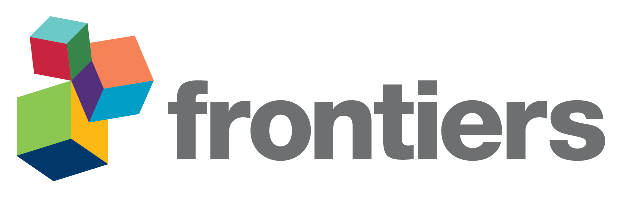
\includegraphics[width=10cm]{logo1}% This is a *.eps file
%\end{center}
%\caption{ Enter the caption for your figure here.  Repeat as  necessary for each of your figures}\label{fig:1}
%\end{figure}


\bibliographystyle{frontiersinSCNS_ENG_HUMS} % for Science, Engineering and Humanities and Social Sciences articles, for Humanities and Social Sciences articles please include page numbers in the in-text citations
%\bibliographystyle{frontiersinHLTH&FPHY} % for Health, Physics and Mathematics articles
\bibliography{../ref/UEH-EVN-Data}

\end{document}
